\documentclass[12pt,oneside]{uhthesis}
\usepackage{subfigure}
\usepackage[ruled,lined,linesnumbered,titlenumbered,algochapter,spanish,onelanguage]{algorithm2e}
\usepackage{amsmath}
\usepackage{amssymb}
\usepackage{amsbsy}
\usepackage{caption,booktabs}
\captionsetup{ justification = centering }
\usepackage{mathpazo}
\usepackage{float}
\setlength{\marginparwidth}{2cm}
\usepackage{todonotes}
\usepackage{listings}
\usepackage{xcolor}
\usepackage{multicol}
\usepackage{graphicx}
\usepackage[utf8]{inputenc}
\usepackage[nodayofweek]{datetime}
\usepackage{hhline}
\usepackage{multirow}

\floatstyle{plaintop}
\restylefloat{table}

\addbibresource{Bibliography.bib}

% \setlength{\parskip}{\baselineskip}%
\renewcommand{\tablename}{Tabla}
\renewcommand{\listalgorithmcfname}{Índice de Algoritmos}
%\dontprintsemicolon

\SetAlgoNoEnd

\definecolor{codegreen}{rgb}{0,0.6,0}
\definecolor{codegray}{rgb}{0.5,0.5,0.5}
\definecolor{codepurple}{rgb}{0.58,0,0.82}
\definecolor{backcolour}{rgb}{0.95,0.95,0.92}

\lstdefinestyle{mystyle}{
    backgroundcolor=\color{backcolour},   
    commentstyle=\color{codegreen},
    keywordstyle=\color{purple},
    numberstyle=\tiny\color{codegray},
    stringstyle=\color{codepurple},
    basicstyle=\ttfamily\footnotesize,
    breakatwhitespace=false,         
    breaklines=true,                 
    captionpos=b,                    
    keepspaces=true,                 
    numbers=left,                    
    numbersep=5pt,                  
    showspaces=false,                
    showstringspaces=false,
    showtabs=false,                  
    tabsize=4
}

\lstset{style=mystyle}


\title{Reconstrucción 3D de la úlcera del pie diabético con cámaras de profundidad Intel\textregistered~RealSense\texttrademark~D435i}
\author{\\\vspace{0.25cm}Ariel Alfonso Triana Pérez\\\vspace{0.2cm}Javier Alejandro Valdés González}
\advisor{\\\vspace{0.25cm}Dr. José Alejandro Mesejo Chiong}
\degree{Licenciado en Ciencia de la Computación}
\faculty{Facultad de Matemática y Computación}
\date{\today\\\vspace{0.25cm}\href{https://github.com/jvaldesgonzalez/dfu\_thesis}{github.com/jvaldesgonzalez/dfu\_thesis}}
\logo{Graphics/uhlogo}
\makenomenclature

\renewcommand{\vec}[1]{\boldsymbol{#1}}
\newcommand{\diff}[1]{\ensuremath{\mathrm{d}#1}}
\newcommand{\me}[1]{\mathrm{e}^{#1}}
\newcommand{\pf}{\mathfrak{p}}
\newcommand{\qf}{\mathfrak{q}}
%\newcommand{\kf}{\mathfrak{k}}
\newcommand{\kt}{\mathtt{k}}
\newcommand{\mf}{\mathfrak{m}}
\newcommand{\hf}{\mathfrak{h}}
\newcommand{\fac}{\mathrm{fac}}
\newcommand{\maxx}[1]{\max\left\{ #1 \right\} }
\newcommand{\minn}[1]{\min\left\{ #1 \right\} }
\newcommand{\lldpcf}{1.25}
\newcommand{\nnorm}[1]{\left\lvert #1 \right\rvert }
\renewcommand{\lstlistingname}{Ejemplo de código}
\renewcommand{\lstlistlistingname}{Ejemplos de código}

\begin{document}

\frontmatter
\maketitle

\begin{dedication}
    \textit{Dedicación}
\end{dedication}
\begin{acknowledgements}
A mi padre celestial, Dios, pues me ha dado la oportunidad a llegar hasta aquí siendo guiado por su mano.

A mi esposa amada, Susy, por soportar mis cargas, por ser mi ayuda idónea cada día, por meterse conmigo en el desarrollo del trabajo.

A mi papá y mi mamá, por instruirme en el camino del bien, y apoyarme en cada etapa. A mi hermano que no existía día o noche que no preguntara cómo me iba.

A todos los amigos que hice en el viaje universitario; en especial, a mi hermano Toledo, hoy llegamos hasta aquí dando cada paso juntos, aprendiendo codo con codo las materias de la carrera.

A Javier y al tutor Alejandro Mesejo, por sus ideas, ayudas, consejos para el desarrollo del trabajo. 

A cada médico con el que trabajamos, cada paciente, y todos aquellos que brindaron su tiempo y recursos en el trabajo.

A los hermanos de la fe, pues conozco que sus oraciones no fallaron.

\begin{flushright}
	Ariel Alfonso Triana Pérez
\end{flushright}

Las primeras palabras de agradecimiento siempre irán dirigidas a mis padres, por su amor, sus consejos y sus peleas también. Por ser la razón principal de lo que soy.

A mis amigos, a esos que vienen conmigo desde el principio, y que todavía no nos aburren los mismos cuentos de siempre... y ojalá nunca lo hagan.

A ``la jungla'', que de una forma u otra siempre está presente en todo.

A Adriana, por acompañarme en el camino y aguantar todas mis malas caras y contestas, que en este tiempo fueron bastante.

A mi profesora y entrenadora Marifelis Portuondo, por mostrarme el mundo de la ciencia desde temprano, gracias MamáFelix.

A mi compañero Ariel, y mi tutor Alejandro Mesejo, por las buenas ideas, el apoyo y la oportunidad de realizar a su lado este trabajo.

\begin{flushright}
	Javier Alejandro Valdés González
\end{flushright}
\end{acknowledgements}
\begin{opinion}

La Diabetes Mellitus es una de las cuatro principales enfermedades crónicas no transmisibles que ocupan las agendas de salud en todo el planeta. Entre las múltiples afectaciones a la salud humana que provoca se encuentran las úlceras en las extremidades inferiores que pueden ocurrir en el 15-35\% de la población diabética en algún momento de su vida. Estas úlceras, conocidas como úlceras de pie diabético (UPD), son causantes del 80\% de las amputaciones por causas no traumáticas de extremidades inferiores. Las UPD son reconocidas como un serio y costoso problema de salud.
    
Uno de los pasos esenciales para el tratamiento efectivo de las UPD es la evaluación progresiva de su severidad. Para esto se han desarrollado diferentes métodos. Casi todos incluyen entre los criterios a evaluar la medición del área y el volumen de la UPD. Evidentemente disponer de un método eficiente y no invasivo para estas mediciones es fundamental para la evaluación del tratamiento de las UPD. El sistema de salud cubano actualmente carece de un sistema efectivo para la medición de las UPD, aquí radica la extrema relevancia del presente trabajo de diploma. 
    
Ariel Alfonso Triana Pérez y Javier Alejandro Valdés González acometieron esta propuesta investigativa con entusiasmo. La aproximación inicial de ambos a la misma estuvo lejos del idílico \textquotedblleft trabajo de mesa\textquotedblright . Tuvieron que asistir con regularidad durante al menos dos meses a la consulta y la sala del Instituto de Angiología y Cirugía Cardiovascular para tomar videos con cámaras RGB-D de las UPD de pacientes tratados en dicha institución. De forma simultánea fueron estudiando temas avanzados del procesamiento de imágenes y la visión computacional mientras intentaban lograr el manejo eficiente de cámaras de profundidad, en específico la Intel\textregistered~RealSense\texttrademark~D435i. Esto lo lograron con suma independencia y todo el rigor necesario. Lograron añadir a su bagaje científico conceptos como stereo vision, depth sensing, object tracking, 3D reconstruction, image segmentation y mesh processing entre muchos otros.

El resultado satisfactorio del trabajo de Ariel y Javier, a pesar del desafío impuesto, era de esperarse dada la adición de rigor investigativo con perseverancia en la solución de problemas mostrada por ambos. El prototipo logrado es una excelente primera aproximación al desarrollo de un sistema eficiente de medición 3D de UPD para el sistema cubano de salud. Es más de lo que pensé era alcanzable en el corto plazo concedido para la investigación. Considero que Ariel Alfonso Triana Pérez y Javier Alejandro Valdés González muestran con amplitud la calidad que se espera de un egresado de Ciencia de la Computación de nuestra Facultad. Recomiendo, con suma satisfacción basada tanto en la calidad del sistema propuesto como del trabajo escrito, que se les conceda a ambos la máxima calificación en su ejercicio de culminación de estudios.

\vspace{1cm}

\begin{flushleft}
Dr. José Alejandro Mesejo Chiong

La Habana, 27 de noviembre de 2022.
\end{flushleft} 


\end{opinion}
\begin{resumen}
	La úlcera del pie diabético (UPD) es una herida crónica presentada por el 85\% de los pacientes con diabetes mellitus. Los especialistas necesitan un método objetivo para la evaluación de las heridas para decidir si el tratamiento actual es adecuado o requiere modificaciones. La medición precisa es una tarea importante en el tratamiento de heridas crónicas, porque los cambios en los parámetros físicos de la herida son indicadores del progreso de curación. En este trabajo se explora la viabilidad de utilizar las cámaras RGB-D Intel\textregistered~RealSense\texttrademark~para detectar, segmentar, reconstruir y medir heridas crónicas en 3D. La herida se detecta de forma semi-automática, seleccionando una región de interés. El procedimiento de segmentación de heridas  propone un conjunto de redes neuronales convolucionales funcionando de ensemble para segmentar la zona de la UPD . Se utiliza el framework \textit{Open3D} para la reconstrucción de la herida, integrando la escena con el resultado de la segmentación. El sistema resultante proporciona un modelo 3D en color preciso de la herida segmentada y permite al usuario obtener estimaciones del volumen, el área y el perímetro de la herida, lo que ayuda en la selección de una terapia adecuada.
\end{resumen}

\begin{abstract}
	Resumen en inglés
\end{abstract}
\tableofcontents
\listoffigures
\listoftables
% \listofalgorithms
% \lstlistoflistings

\mainmatter

\chapter*{Introducción}\label{chapter:introduction}
\addcontentsline{toc}{chapter}{Introducción}

La diabetes mellitus se define, según la Asociación Americana de Diabetes (ADA, por sus siglas en inglés), como una enfermedad metabólica caracterizada por hiperglucemia crónica, resultado de un déficit de la hormona insulina, la resistencia a esta o de ambas causas. Según \textit{Diabetes Atlas} en el año 2021, uno de cada siete adultos vivía con diabetes en América del Norte y el Caribe, mientras que uno de cada diez adultos vivía con la enfermedad en América Central y del Sur \cite{diabetesAtlas}. Por otra parte, según el \textit{Anuario Estadístico de Salud de Cuba}, la prevalencia de esta enfermedad en el país al finalizar el 2020, era de 66.9 por cada 1000 habitantes \cite{anuario2020}, con un incremento del 2.6 con respecto al año 2018 \cite{anuario2018}.

La diabetes mellitus es la enfermedad endocrina incurable más extendida y ocupa el tercer lugar entre las dolencias más serias que enfrenta la humanidad. El sistema cardiovascular suele afectarse precozmente en el diabético, causando infartos silenciosos, miocardiopatía diabética e hipertensión. Este padecimiento afecta en su proceso degenerativo diferentes estructuras oculares, causando retinopatía diabética la cual es el principal desencadenante de ceguera. La diabetes tiene manifestaciones renales infeccionas (pielonefritis y cistitis) y no infecciosas (nefropatía diabética), además daña el sistema nervioso periférico causando neuropatía diabética, parálisis de los nervios craneales y coma hiperosmolar diabético. La hiperglucemia en el diabético produce diversas alteraciones cutáneas, son frecuentes las infecciones por diversos gérmenes y hongos. El daño de los pequeños y grandes vasos produce atrofia de la piel que junto con la neuropatía, constituyen el terreno adecuado para la formación de úlceras en los pies. El seguimiento de esta enfermedad constituye uno de los temas de salud más importantes, debido a su prevalencia, consecuencias físicas y psicosociales \cite{roca}.

En medicina, se considera que el pie diabético son todas las lesiones que las personas diabéticas presentan en los pies, por debajo del maléolo~\footnote{Protuberancias con forma vagamente semiesférica que anatómicamente forman parte de la articulación del tobillo.}, causadas por disímiles desórdenes. Se conoce que el 85 \% de los pacientes que sufren amputaciones han padecido una úlcera del pie diabético \footnote{Llaga o herida abierta que generalmente se produce en la planta del pie.} (UPD). La duración de las úlceras puede variar desde pocas semanas hasta incluso años. Los diabéticos enfrentan un notable detrimento de su calidad de vida. 

En la actualidad los médicos cubanos utilizan varios protocolos de tratamientos para curar las lesiones. El principal tratamiento empleado es el Heberprot-P~\textregistered \cite{berlanga2013heberprot} un producto que favorece la cicatrización de la UPD y reduce el riesgo de amputación. Hasta la fecha, cerca de 20 000 casos con UPD han recibido sus beneficios como parte del ``Programa de Atención Integral al Paciente con UPD con el uso del Heberprot-P'' \cite{gonzalez2015resultados}. Otro de los tratamientos utilizado es la ozonoterapia que presenta resultados favorables para el 75 \% de los pacientes~\cite{alvarez2014beneficios}, además esta medida terapéutica ha sido combinada con el uso del Heberprot-P~\textregistered arrojando mejores resultados que los tratamientos por separado~\cite{martinez2019evolucion}. A pesar de todos estos tratamientos y estudios, los galenos cubanos no cuentan con una herramienta cuantitativa efectiva que valore la severidad y el proceso de curación de la UPD. La evaluación clínica depende en gran medida de las habilidades del experto para determinar un criterio acertado sobre la evolución del paciente. Actualmente, la evaluación clínica se establece según la opinión de tres especialistas que examinan al paciente y toman decisiones en conjunto. Bajo estas circunstancias, la aplicación de un diagnóstico y una terapia adecuada se ven retrasadas.

En base a esta problemática se han realizado numerosos trabajos investigativos dirigidos al desarrollo de métodos y aplicaciones para la medición precisa de la UPD. Una de las formas adoptadas para la medición, es la toma de imágenes fotográficas de la lesión, por ejemplo utilizando una cámara acoplada al FrameHeber 03 \cite{cabal2019quantitative}, un dispositivo desarrollado en el Centro de Ingeniería Genética y Biotecnología que ya no se encuentra en uso o producción. El FrameHeber 03 tuvo entre sus inconvenientes que debía esterilizarse cada vez que se empleaba, lo que retrasaba el flujo de pacientes en las consultas. 

Se tienen registros de trabajos que luego de la toma de las imágenes fotográficas, aplicaban distintas técnicas de segmentación de la zona donde se presenta la úlcera \cite{garcia2019mejoramiento, pena2016segmentacion, heras2022diabetic, ching2022segm3d}. En \cite{garcia2019mejoramiento} se concluye que se puede incluir el algoritmo de mezclas gaussianas para la segmentación automática de la DFU en un software para realizar las mediciones. En  \cite{pena2016segmentacion} se propone un sistema semiautomático que utiliza transformaciones de espacios de color para la segmentación. Heras en \cite{heras2022diabetic} desarrolló el sistema \emph{DFUlcer-UH: Annotation Tools}, que incluye un módulo de segmentación de los bordes de la úlcera utilizando una regresión logística y operadores morfológicos, además incluye segmentación de los tejidos internos de la úlcera utilizando el algoritmo \textit{Density Based Spatial Clustering of Applications with Noise} (DBSCAN). Mientras que en \cite{ching2022segm3d} se propone una red neuronal entrenada para la segmentación de los bordes de la UPD.

La evolución de la UPD por lo general, ocurre con la granulación de la lesión en primer lugar, lo cual conlleva un cambio de volumen, seguido por la cicatrización que se traduce en un decremento gradual del área y el perímetro de la lesión  \cite{kecelj2007measurement}. Se han desarrollado trabajos que permiten medir el área y el perímetro de la lesión con técnicas invasivas como la planimetría, sea digital o mecánica \cite{oien2002measuring}, donde se coloca un papel cuadriculado sobre la úlcera y se marca el borde para luego realizar las mediciones. Para la estimación del volumen se conocen dos técnicas invasivas que consisten en rellenar la cavidad con solución salina o con pasta de silicio y luego calcular el volumen de los materiales \cite{langemo2008measuring}. Estos métodos invasivos pueden provocar infecciones en los pacientes, incitando un retroceso en el proceso de sanación. Dentro de este contexto la reconstrucción 3D y el procesamiento de imágenes brindan opciones no invasivas. La reconstrucción 3D consiste en la representación de la escena mediante mallas poligonales utilizando información de profundidad y de color.

Se han desarrollado dos acercamientos principales a la modelación y reconstrucción 3D de las úlceras: la visión pasiva y activa \cite{zenteno2018volumetric}. La visión pasiva es aquella que directamente detecta la luz presente en la escena sin necesidad de utilizar fuentes luminosas externas \cite{malian2004medphos, plassmann1998mavis}. Por otra parte, la visión activa emplea una fuente invisible infrarroja para iluminar la escena (i.e. técnica de luces estructuradas \cite{filko2018wound, ching2022segm3d, ozturk1996new} o escáneres láseres \cite{callieri2003derma, krouskop2002noncontact}). Con la creciente prevalencia de los teléfonos inteligentes y tablets con alta resolución se han presentado trabajos con atractivas opciones para la evaluación de las UPD \cite{foltynski2014new, wang2014smartphone}. Sin embargo, muchas de estas propuestas tienen un alto precio por lo que dejan de ser factibles para los hospitales cubanos y/o son complejos de utilizar para el tratamiento rutinario en centros hospitalarios.

\section*{Objetivos}

Nuestro objetivo es diseñar un sistema de bajo costo, práctico y que no sea invasivo para el paciente, que permita tomar mediciones de las úlceras utilizando las cámaras de profundidad Intel~\textregistered RealSense™ D435i y técnicas de reconstrucción 3D. El sistema debe medir perímetro y área (como indicadores de la cicatrización de la lesión), y volumen (como estimador de la granulación). Las mediciones deben ser estables en el tiempo. Esta tesis propone un sistema que automatiza la segmentación 2D, reconstrucción 3D y medición de las UPD a partir de imágenes RGB-D. Dicho proceso funciona de la siguiente forma: 

\begin{enumerate}
	\item Para la captura de la secuencia se utiliza una cámara RGB-D~\footnote{Una cámara RGB–D es una cámara que capta imágenes a colores (RGB - formato \textit{Red} (rojo), \textit{Green} (verde), \textit{Blue} (azul)) y tiene sensor de profundidad (D - \textit{depth} (profundidad)).}.
	\item Se posprocesa la secuencia mejorando el contraste de las imágenes, aplicando filtros de enfoque y otras operaciones.
	\item Luego, se emplean 10 Redes Neuronales Convolucionales, funcionando en conjunto utilizando el promedio, se segmentan las imágenes RGB que resultan en máscaras binarias.
	\item Posteriormente, se aplican operadores morfológicos y otras operaciones a las máscaras para eliminar ruido resultante de la predicción.
	\item Antes de medir, se procede a realizar la reconstrucción 3D utilizando las máscaras.
\end{enumerate}


En consecuencia, el modelo 3D final consiste en una malla que representa de la forma más precisa posible solo la superficie de la región que ocupa la UPD. Una vez obtenido el modelo 3D de la úlcera, se procede a realizar las estimaciones de perímetro, área y volumen.

Para lograr el objetivo general se proponen objetivos específicos mencionados a continuación:

\begin{enumerate}
	\item Creación de un conjunto de muestras de UPD que contenga videos grabados con la cámara RGB-D para la validación de la segmentación, reconstrucción y medición de las lesiones.
	\item Elaborar el sistema de segmentación, reconstrucción 3D y medición de la herida con del uso de la cámara RGB-D. Aplicar técnicas de pre/posprocesamiento para mejorar la calidad de los resultados.
	\item Analizar el desempeño de los resultados obtenidos respecto a la segmentación manual del conjunto de datos.
\end{enumerate}

Para cada uno de los propósitos específicos de este tema se combinarán una serie de técnicas y algoritmos cuidadosamente seleccionados de la previa revisión bibliográfica. Lográndose así, un nuevo sistema de segmentación, reconstrucción 3D y medición con el uso de una cámara RGB–D Intel~\textregistered RealSense™ D435i.

\section*{Organización de los Capítulos}

Esta tesis cuenta con un total de 4 Capítulos. En el Capítulo 1 se expone la revisión de la literatura donde se presentan algunos de los algoritmos existentes en las problemáticas descritas. El Capítulo 2 explica de forma breve los fundamentos teóricos, necesarios para la comprensión del trabajo. El Capítulo 3 da a conocer la estructura general de la propuesta final y una explicación de la selección de los algoritmos en las diferentes fases. Luego, en el Capítulo 4 se presentan los resultados obtenidos y se comparan con los de otros sistemas. Posteriormente, se dan las conclusiones y recomendaciones de la investigación con el propósito de su continuación. Para finalizar, se adjunta la bibliografía del trabajo.
\chapter{Estado del Arte}\label{chapter:state-of-the-art}


\chapter{Marco Teórico}\label{chapter:theoretical-framework}


En el presente capítulo se brinda una breve explicación de los conceptos tenidos en cuenta durante el desarrollo del trabajo. En la Sección \ref{section:rgbd} se presentan los principios de la tecnología RGB-D y funcionamiento de las cámaras de profundidad, en particular la Intel~\textregistered RealSense™ Depth Camera D435i. En la Sección \ref{section:imgEnh} se presentan los fundamentos básicos de mejoramiento de imágenes empleados en la investigación. Por otro lado, en la Sección \ref{section:tracking} se explican los algoritmos de seguimiento de objetos en muestras de video. En la Sección \ref{section:seg} se detallan los principios y algoritmos de segmentación en imágenes RGB. La Sección \ref{section:rec3d} aborda los algortimos y etapas de la reconstrucción 3D utilizando imágenes de profundidad. Posteriormente, en la Sección \ref{section:measure} se sientan las bases de las mediciones de perímetro, área y volúmen de mallas y nubes de puntos 3D.

\section{Tecnología RGB-D}\label{section:rgbd}

En el campo de visión por computadoras la estructura de datos más empleada es la imagen. Una imagen permite almacenar una porción del entorno en un instante determinado.

\begin{definition}\label{def:img}
	Se define una imagen $I_{n \times m}$ como un arreglo bidimensional con $n$~filas y $m$ columnas, tal que $I_{n \times m}[i, j] = p_{i,j}$ es un píxel y se cumple que $p_{i, j} \in \mathbb{N}^k: 0~\leq~i~\leq~n -1 \wedge 0 \leq j \leq m - 1 \wedge k \in \mathbb{N}$.
\end{definition}

\begin{definition}
	Se define un píxel $p_{i, j} \in \mathbb{N}^k: k \in \mathbb{N}$ como el vector en la posición $i, j$ de la imagen $I_{n \times m}: 0 \leq i \leq n -1 \wedge 0 \leq j \leq m - 1$
\end{definition}

El valor $k$ varía en dependencia del espacio de color en el cual se tome la imagen u otras características adicionales que se asocien a cada píxel. A continuación se describen los espacios de color utilizados en la propuesta:

\begin{itemize}
	\item \textbf{RGB} es uno de los espacios de colores más populares utilizados en la segmentación de imágenes, está basado en la teoría tri-cromátrica, y por lo tanto define a cada color como una combinación de los tres colores primarios (rojo, verde y azul). Este espacio se define geométricamente como un cubo en donde cada coordenada puede tomar valores desde 0 hasta 255~\cite{sangwine1998colour}. Se considera que 	este espacio de color es dependiente del dispositivo con el que se capture	la foto~\cite{tkalcic2003colour}~\cite{ruela2013role}. Este espacio aporta tres componentes: [R, G, B], o sea, el valor $k$ de la Definición \ref{def:img} vale 3.
	\item \textbf{HSV} es una transformación de las coordenadas rectangulares de RGB a cilíndricas. En este espacio cilíndrico, cada color está representado por una combinación de matiz (H), saturación (S) y brillo (V). El matiz es la coordenada angular y varía de $0^{\circ}$ a $360^{\circ}$. La saturación es la cantidad de color puro presente en la región con respecto a la cantidad de blanco, esta varía entre 0 y 1. Finalmente, el brillo, mide la cantidad de blanco presente en el color y varía de 0 a 255~\cite{ruela2013role}. Este espacio aporta igualmente tres componentes: [H, S, V].
	\item \textbf{L*A*B} El espacio de color L*a*b* resulta de una transformación no lineal del espacio RGB~\cite{bradski2000opencv}. L* representa el brillo, mientras a* y b* representan el matiz y la saturación de un color. En este espacio de color L* se desplaza de negro a blanco, mientras a* se desplaza desde verde a rojo y b* desde azul a amarillo. Este espacio aporta tres componentes: [L, A, B].
	\item \textbf{YCbCr} Es una familia de espacios de color utilizadas en sistemas de video. Y es la luminancia, mientras Cb y Cr son las componentes de crominancia azul y roja respectivamente~\cite{sergyan2007color}. Este espacio aporta tres componentes: [Y, Cb, Cr].
\end{itemize}

Una imagen en cualquiera de los espacios anteriores brinda información del entorno, de los objetos que pertenecen al mismo, del instante de tiempo en que fue tomada por una cámara, pero no de la distancia a la que se encuentran los objetos presentes en la imagen.

\begin{definition}
	Una imagen RGB-D se define como una imagen $I_{n \times m}$ en el espacio RGB con $n$ filas y $m$ columnas, y una matriz $D \in M_{n, m}$ donde $D[i, j]: 0~\leq~i~\leq~n \wedge 0~\leq~j~\leq~m$ representa la distancia a la que se encuentra el píxel $p_{i,j} \in I_{n \times m}$ de la cámara.
\end{definition}

Las imágenes RGB-D brindan suficiente información sobre los entes presentes en el entorno y permiten realizar reconstrucciones en tres dimensiones de las escenas de forma precisa. 

\subsection{Cámaras de profundidad}

Las cámaras son herramientas esenciales en el campo de visión computacional. La salida de las cámaras digitales tradicionales son imágenes en 2D, donde cada píxel es un vector en el espacio de color correspondiente, por lo general en RGB. Una cámara de profundidad toma imágenes compuestas por píxeles con valores númericos asociados diferentes. En el caso de las cámaras de profundidad el valor asociado corresponde a la distancia de la cámara o la profundidad. Algunas de estas herramientas tienen ambos sistemas RGB y de profundidad, los cuales producen imágenes con píxeles que tienen estos cuatro valores.

La salida de las cámaras de profundiad pueden ser visualizadas de diversas formas: en la Figura \ref{fig:rgbd} la imagen de color se muestra al lado de la imagen de profundidad, donde cada color diferente en el mapa de profundidad representa una distancia de la cámara.

\begin{figure}[h]
	\centering
	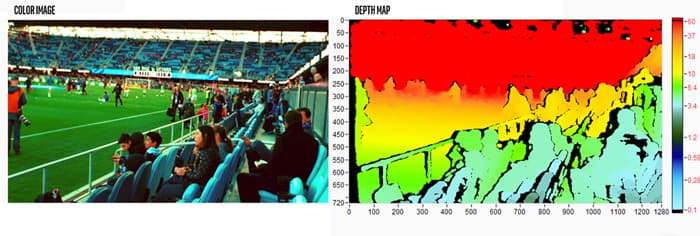
\includegraphics[width=10cm]{./Graphics/rgbd.png}
	\caption{Imagen de color e imagen de profundidad. El color cyan en el mapa de profundidad corresponde a las distancias más cercanas. Tomado de \cite{intel}.}
	\label{fig:rgbd}
\end{figure}

\subsubsection{Tipos de cámaras}

Existe una gran variedad de métodos para calcular profundidad, cada uno de ellos con sus fortalezas, debilidades y condiciones ideales de operación. 

\begin{itemize}
	\item \textbf{Luz estructurada y codificada:} Las cámaras de profundidad que utilizan estas tecnologías similares proyectan una luz, usualmente luz infrarroja desde un emisor hacia la escena. La luz proyectada es un patrón visual, de tiempo o una combinación de estos. El sensor en la cámara detecta el patrón proyectado en la escena y recibe información de profundidad producto de la deformación. 
	
	Por ejemplo si el patrón consiste en una serie de líneas que se proyecta sobre una pelota, entonces las líneas deben deformarse alrededor de la superficie de la pelota de una forma específica. Si la pelota se acerca al emisor, el patrón cambia de igual forma. Utilizando la diferencia entre la imagen esperada y la imagen captada por la cámara, entonces se puede calcular la distancia hasta la cámara de cada píxel.
	
	\item \textbf{Profundidad estéreo:} Las cámaras de profundidad estéreo a menudo proyectan luces infrarrojas hacia la escena para mejorar la precisión de los datos. Las cámaras estéreo utilizan cualquier luz para medir profundidad. Estas herramientas tienen dos sensores colocados a una distancia pequeña denominada \textit{baseline}. La cámara toma dos imágenes desde los sensores y las compara, dado que el \textit{baseline} es un valor fijo y conocido, esta comparación entre las imágenes aporta información de profundidad. Estos dispositivos funcionan similar al cerebro y los ojos. Objetos cercanos se mueven significativamente de un ojo a otro, mientras que objetos lejos se mueven muy poco. 
	
	\item \textbf{Tiempo de vuelo y LiDAR} Todas las tecnologías anteriormente descritas se apoyan en información conocida para calcular profundidad. Los sensores LiDAR son un tiempo de cámaras que utilizan luz láser para calcular profundidad. Emiten una luz sobre la escena y calculan cuanto demora a la luz volver al sensor de la cámara. En dependencia del poder y longitud de onda de la luz, estos sensores se pueden emplear para medir distancias significativas.
\end{itemize}
\subsection{Matriz intrínseca de la cámara}

El trabajo teórico con estos dispositivos requiere del diseño de modelos que representen y simulen su comportamiento real. Por este motivo, la literatura abarca diversos esquemas de complejidad variable que describen los distintos tipos de cámaras existentes. Este proyecto se centra en el \textit{modelo de proyección general}, que constituye una generalización que elimina las restricciones sobre todos los parámetros del \textit{modelo de cámara estenopeica} conocida por su nombre en inglés pinhole camera.

\begin{definition}
	La matriz del modelo de cámara de proyección general P transforma puntos $\hat{X} = [X, Y, Z]^T$ del mundo real a puntos $\hat{x} = [x, y]^T$ de la imagen según $\hat{X} = P\hat{x}$, siendo $\bar{X} = [X, Y, Z, 1]^T$ el vector extendido de $\hat{X}$ y $\bar{x} = [x, y, 1]^T$ el vector extendido de $\hat{x}$. La matriz P es de dimensión $3 \times 4$ de rango 3, conocida como matriz de la cámara o de proyección y puede factorizarse de la forma~\cite{hartley2004camera}:
	\begin{equation}\label{eq:proyGeneral-1}
		P = KR[I| - C] = K[R|t]
	\end{equation}
	\begin{equation}\label{eq:proyGeneral-2}
		t = -RC
	\end{equation}
	Por tanto,
	\begin{equation}\label{eq:proyGeneral-3}
		\begin{pmatrix}
			x\\
			y\\
			1
		\end{pmatrix} = K[R|t] \begin{pmatrix}
			X\\
			Y\\
			Z\\
			1	
		\end{pmatrix}
	\end{equation}
\end{definition}

\begin{figure}[h]
	\centering
	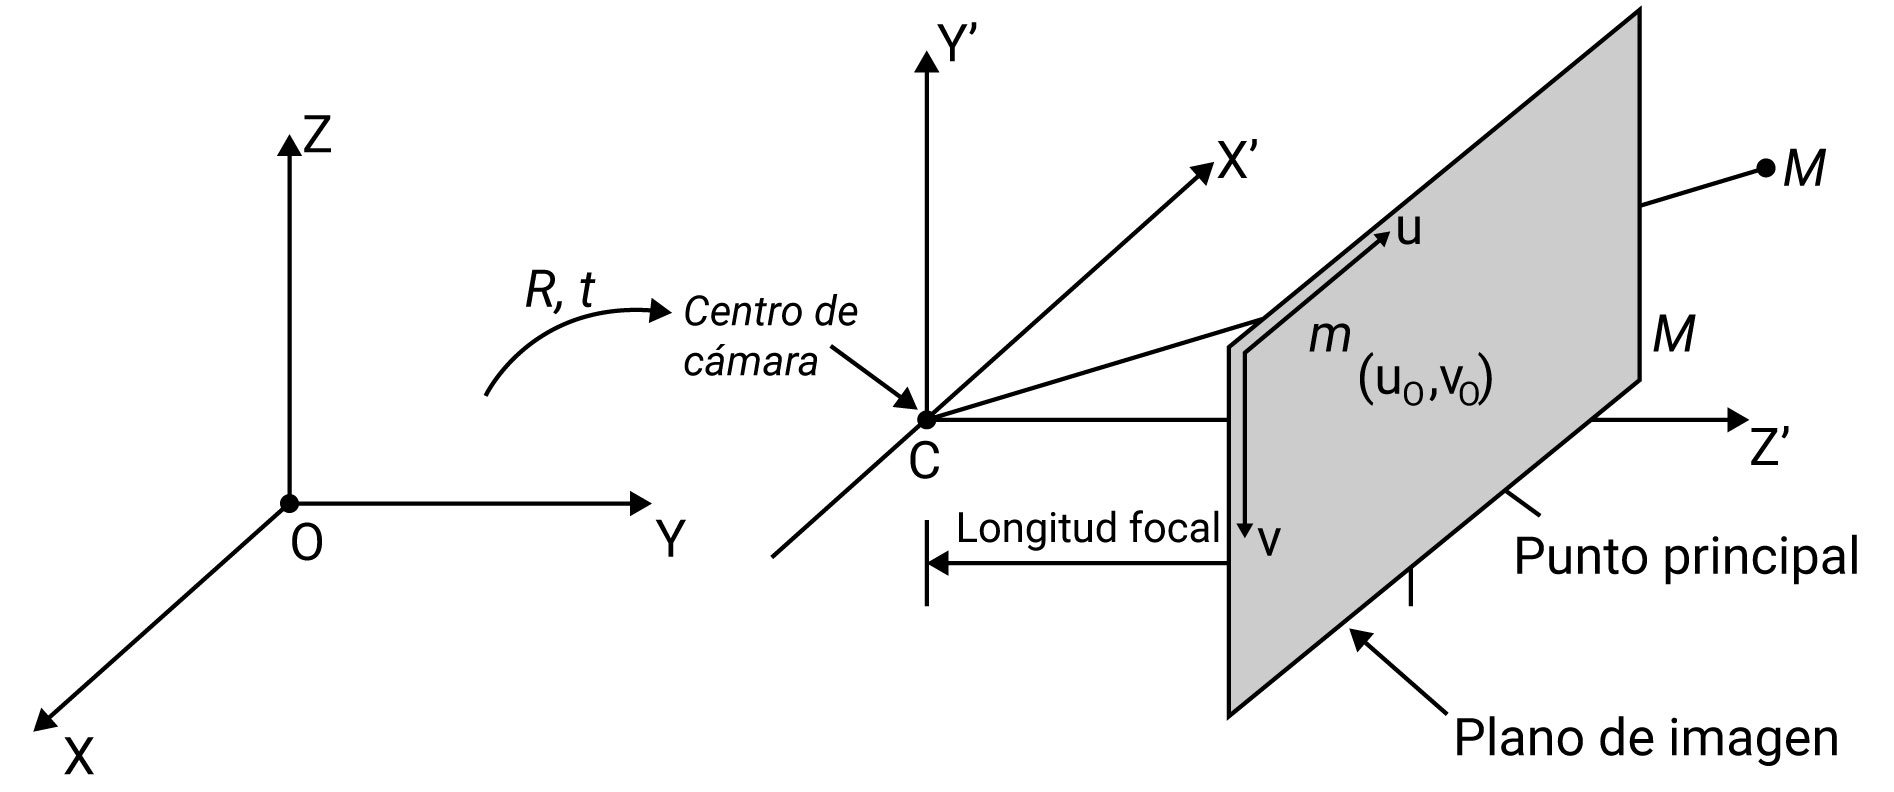
\includegraphics[width=10cm]{./Graphics/modelo-proyeccion-general.png}
	\caption{Modelo de cámara de proyección general. Sistema de coordendas de (a) Objeto o realidad (X, Y, Z), (b) Cámara (X', Y', Z') e (c) Imagen (u, v). Tomada de~\cite{ji2022vision}.}
	\label{fig:proyGeneral}
\end{figure}

En la definición anterior $C$ representa las coordenadas del centro de cámara en el sistema de coordenadas reales (Figura \ref{fig:proyGeneral}(a)) y R es la matriz de rotación de dimensiones $3 \times 3$, que representa la orientación del sistema de coordenadas de la cámara (Figura \ref{fig:proyGeneral} (b)). Los parámetros de R y C son conocidos como externos o de orientación exterior. La notación $[I| - C]$ representa la matriz compuesta por la identidad $I$ junto al vector columna $-C$ y análogamente sucede con $[R|t]$.

La matriz $K$ es conocida como matriz intrínseca o de calibración, la cual es invariante para una misma cámara. Es la encargada de determinar la proyección del sistema de coordenadas de la cámara a coordenadas de la imagen (Figura \ref{fig:proyGeneral} (c)). Como bien su nombre indica está formada por los parámteros internos (intrínsecos) y posee la siguiente estructura:

\begin{equation}
	K = \begin{pmatrix}
		m_x && 0 && 0 \\
		0 && m_y && 0 \\
		0 && 0 && 0 \\
	\end{pmatrix}
	\begin{pmatrix}
		f && \frac{s}{m_x} && p_x \\
		0 && f && p_y \\
		0 && 0 && 1 \\
	\end{pmatrix} =
	\begin{pmatrix}
		a_x && s && x_0 \\
		0 && a_y && y_0 \\
		0 && 0 && 1 \\
	\end{pmatrix}
\end{equation}

donde, $m_x$ y $m_y$ son el número de píxeles por unidades de las coordenadas $x$ y $y$ de la imagen. Por tanto $a_x = fm_x$ y $a_y = fm_y$ constituyen la distancia focal $f$ representada en número de píxeles respecto a las direcciones $x$ y $y$. De igual manera ($x_0 = p_xm_x, y_0 = p_ym_y$) son las coordenadas del punto principal $(p_x, p_y)$ en términos de número de píxeles. $s$ (skew), indica la desviación de rectangularidad. Sin embargo, para cámaras usuales se asume $s=0$.

Tanto los parámetro internos como los externos son adquiridos a partir de la calibración geométrica del sistema.

\begin{definition}
	La calibración geométrica es el proceso de determinación de las propiedades geométricas de la cámara. Su propósito es descubrir la correspondencia entre rayos y puntos de la imagen~\cite{kannala2008geometric}.
\end{definition}

El método de calibración que se detalla a continuación, basado en técnicas convencionales para modelos de proyección general, fue extraído de \cite{zhang2000flexible}. A diferencia de otros procedimientos solo requiere de la cámara para observar un patrón plano desde diferentes orientaciones.

\subsubsection{Método de calibración}

De manera general, a partir de las imágenes de un objeto de calibración, se comienza con una solución analítica de los parámetros y luego se aplica una técnica de optimización no lineal basada en el criterio de máxima similitud.

\begin{enumerate}
	\item Captura de imágenes del objeto de calibración y detección de sus puntos de control.
	
	En el caso del modelo de proyección general, la matriz de la cámara está representada por P como se describe en la ecuación \ref{eq:proyGeneral-1}. Dado que el objeto de calibración que se utiliza es plano (Figura \ref{fig:chess}) y todos los parámetros en $K$ son desconocidos, se necesita la captura de varias imágenes con diferente orientación. Las propiedades geométricas del objeto de calibración se conocen, por tanto, una vez obtenidas las imágenes se procede a detectar los puntos de control.
	
	\begin{figure}[h]
		\centering
		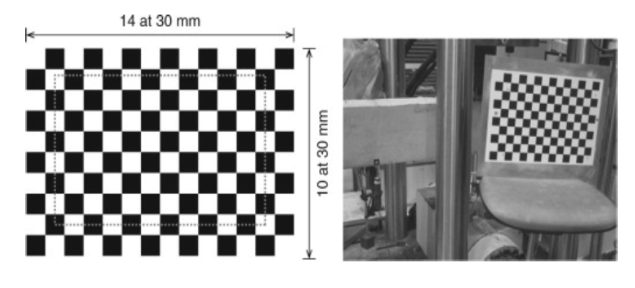
\includegraphics[width=10cm]{./Graphics/chess.png}
		\caption{Calibración basada en objetos planos. Tomada de \cite{ching2022segm3d}}
		\label{fig:chess}
	\end{figure}
	\item Estimación de los parámetros intrínsecos y extrínsecos.
	
	La correspondencia entre un plano de la escena y su imagen de perspectiva es una homografía plana~\footnote{Homografía plana, relación lineal entre las coordenadas de los puntos en un plano arbitrario de la escena y las coordenadas de esos puntos en la imagen.}. Sin pérdida de la generalidad se asume que el plano de calibración es $Z = 0$ y se denota la $i$-ésima columna de la matriz de rotación $R$ por $r^i$. De la ecuación \ref{eq:proyGeneral-3} se tiene:
	
	\begin{equation}
		\begin{pmatrix}
			x\\
			y\\
			1
		\end{pmatrix} = K[r^1|r^2|r^3|t] \begin{pmatrix}
			X\\
			Y\\
			0\\
			1
		\end{pmatrix}
		= K[r^1|r^2|t]
		\begin{pmatrix}
			X\\
			Y\\
			1
		\end{pmatrix}
		= H\begin{pmatrix}
			X\\
			Y\\
			1
		\end{pmatrix}
	\end{equation}
	donde la matriz $3 \times 3$ de homografía es:
	\begin{equation}\label{eq:homografia}
		H = K[r^1|r^2|t]
	\end{equation}
	
	Las homografías pueden ser estimadas de múltiples formas dada una imagen del objeto de calibración. En \cite{zhang2000flexible} se presenta una técnica basada en el criterio de máxima similitud, sin embargo, no se profundizará en su explicación. Expresando las columnas de $H$ como $h_i$, usando el hecho de que $r^1$ y $r^2$ son ortonormales y simplificando la notación de $(K^{-1})^T$ como $K^{-T}$ de la ecuación \ref{eq:homografia} se obtiene:
	
	\begin{equation}\label{eq:hom-1}
		h_1^TK^{-T}K^{-1}h_2 = 0
	\end{equation}
	\begin{equation}\label{eq:hom-2}
		h_1^TK^{-T}K^{-1}h_1 = h_2^TK^{-T}K^{-1}h_2
	\end{equation}
	
	Por tanto cada homografía provee dos restricciones que pueden escribirse como ecuaciones lineales de los elementos de la matriz homogénea y simétrica $w = K^{-T}K^{-1}$. Por tanto, el sistema que deriva de las ecuaciones \ref{eq:hom-1} y \ref{eq:hom-2} tiene la forma $Av = 0$, donde el vector de incógnitas $v = (w_{11}, w_{12}, w_{13}, w_{22}, w_{23}, w_{33})^T$ consiste en los elementos de $w$. La matriz $A$ tiene $2N$ columnas donde $N$ es el número de imágenes capturadas. La cantidad de imágenes debe ser mayor o igual que 3. Cuando se resuelve $w$, se puede computar la matriz triangular superior $K$ por la factorización de Cholesky. Dados $K$ y $H$, los parámetros externos pueden ser recuperados de la ecuación \ref{eq:homografia}.
	
	\item Refinamiento de los parámetros.
	
	Finalmente, los parámetros obtenidos se refinan mediante optimización no lineal. La función de costo normalmente usada en la minimización, dadas $n$ imágenes y $m$ puntos del objeto planar, es:
	
	\begin{equation}
		\sum_{i=1}^n\sum_{j=1}^m \|x_{ij} - \bar(K, R_i, t_i, X_j)\|^2
	\end{equation}

	Donde $x_{ij}$ contiene las medidas de las coordenadas del punto de control $j$ en la imagen $i$ y $\bar{x}(K, R_i, t_i, X_j)$ es la proyección del punto de control $X_j$ en la imagen $i$. Este problema de mínimos cuadrados es resuelto con el algoritmo Levenberg-Marquardt~\cite{more1978levenberg}.
\end{enumerate}

\section{Mejoramiento de imágenes. Pre/postprocesamiento}\label{section:imgEnh}

Una de las principales tareas en el procesamiento de imágenes es el mejoramiento de estas con el fin ajustarla digitalmente para su visualización o proveerlas como entrada a algortimos. Entre las técnicas de mejoramiento de imágenes se encuentra la eliminación de ruido, el mejoramiento de contraste, aplicación de filtros y operadores morfológicos, y manipulación del histograma.

Para las explicaciones teóricas de la presente sección considere las imágenes en escala de grises. Todas las operaciones y explicaciones pueden ser extendidas a imágenes RGB aplicándolas en cada canal de color.

\begin{definition}
	El histograma de una imagen $I_{n \times m}$ se define como la función de distribución de los niveles de intensidad de la imagen.
\end{definition}

\subsection{Mejoramiento de contraste: CLAHE}

A menudo, los objetos presentes en las imágenes no se diferencian entre ellos, producto del bajo contraste en la fotografía. Existen técnicas para ajustar los niveles de contraste en una imagen.

\begin{definition}
	Se define como contraste en una imagen la diferencia de intensidad de gris de los píxeles presentes en la imagen.
\end{definition}

La ecualización del histograma es una de las técnicas que permiten el ajuste del contraste. La ecualización se concibe como una transformación o manipulación de la imagen con el fin de obtener un histograma con distribución uniforme. En teoría, la aplicación de esta operación debería transformar el histograma en otro con una forma perfectamente uniforme sobre todos los niveles de gris. Sin embargo, en la práctica esto no se va a poder conseguir pues se estaría trabajando con funciones de distribución discretas en lugar de continuas. En la transformación, todos los píxeles de un mismo nivel de gris se transformarán a otro nivel de gris, y el histograma se distribuirá en todo el rango disponible separando en lo posible las ocupaciones de cada nivel. El resultado de la ecualización maximiza el contraste de una imagen sin perder información de tipo estructural~\cite{solomon2011fundamentals}, esto es, conservando su entropía~\footnote{La entropía es una medida de la información contenida en una imagen, y los estados de niveles de intensidad de los píxeles.}.

\subsubsection{CLAHE}

La ecualización de histograma produce buenos resultados en el mejoramiento de las imágenes, pero el ruido presente también será mejorado. El algoritmo de Ecualización Adaptativa del Histograma con Limitación de Contraste (CLAHE, por sus siglas en inglés) pretende aportar una solución al problema anterior.

CITAR ART \cite{pizer1987adaptive}

\subsection{Filtros}

\subsection{Morfología matemática}

La palabra ``morfología'' se refiere a la forma y estructura de algún elemento. En el campo del procesamiento de imágenes se puede utilizar para referirse a la forma de una región. La morfología matemática es una metodología basada en la teoría de conjuntos y la topología, que intenta de una manera cuantitativa describir la estructura de objetos en una imagen~\cite{}.

Las operaciones morfológicas fueron originalmente definidas como operaciones sobre conjuntos y han demostrado ser útiles para procesar puntos en un espacio de dos dimensiones. Estas utilizan una estructura conocida como elemento estructurante~\cite{}~\cite{}.

\begin{definition}
	Se define una imagen binaria $B_{h \times w}$ como una imagen, tal que: $B_{h \times w}[i, j] = p_{i, j} \in \{0, 1\}$ y $0 \leq i \leq h - 1$, $ 0 \leq j \leq w-1$.
\end{definition}

\begin{definition}
	Se define un elemento estructurante $S$ como una imagen binaria $S_{a \times b}$ representando un tamaño y forma arbitrario.
\end{definition}

Los elementos estructurantes se utilizan para hacer un proceso similar a la convolución aplicando una operación lógica entre el elemento estructurante $S$ y cada píxel $p_{i, j} \in B_{h \times w}$. El resultado de esta operación se almacena en cada píxel. El efecto que se obtiene dependel del tamaño y la forma del elemento estructurante $S$~\cite{} (Figuras \ref{fig:estructurante} y \ref{fig:kernel}).

\begin{figure}[h]
	\centering
	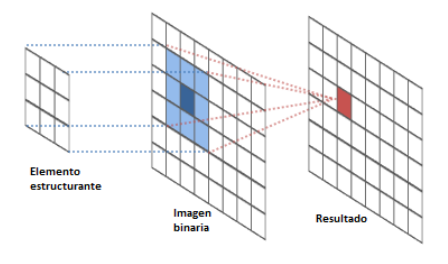
\includegraphics[width=10cm]{./Graphics/estructurante.png}
	\caption{Representación de una operación morfológica con un elemento estructurante}
	\label{fig:estructurante}
\end{figure}	

\begin{figure}[h]
	\centering
	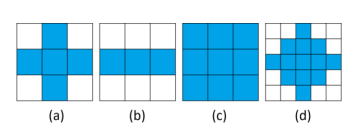
\includegraphics[width=10cm]{./Graphics/kernel.png}
	\caption{Elementos estructurales. (a) cruz, (b) línea, (c) rectángulo de 3$\times$3 y en (d) el disco de radio 2.}
	\label{fig:kernel}
\end{figure}

\subsubsection{Operaciones básicas}

Existen dos operaciones morfológicas básicas de las cuales se obtienen resultados diferentes. Antes de presentarlas se definen algunos conceptos importantes.

\begin{definition}
	Dos píxeles $P_t$ y $P_k$ están conectados si son adyacentes en la imagen en cualquiera de las ocho direcciones.
\end{definition}

\begin{definition}
	Un camino entre un par de píxeles $P_t$ y $P_k$ es una secuencia $P_t = P_1, P_2, \ldots,$ $P_e = P_k$ tal que $P_i$ y $P_{i + 1}$ están conectados $\forall 1 \leq i \leq e$.
\end{definition}

\begin{definition}
	Una región es un conjunto de píxeles conectados de tal forma que entre todo par de píxeles existe un camino.
\end{definition}

\begin{definition}
	Un punto frontera $P_{i, j}$ es un píxel que pertenece a una región pero que al menos uno de sus vecinos no lo está.
\end{definition}

\begin{itemize}
	\item \textbf{Erosión}
	
	La erosión es el proceso de eliminar todos los puntos fronteras de una región, convirtiendo el objeto más pequño en un área por un píxel sobre todo su perímetro. La erosión es útil para remover objetos de una imagen segmentada que pueden ser muy pequeños para ser de interés~\cite{}. En general, se puede definir de la siguiente manera:
	
	\begin{equation}
		E = B \otimes S = \{x, y | S_{x, y} \subseteq B\}
	\end{equation}

	\item \textbf{Dilatación}
	
	La dilatación es el proceso de incorporar a una región todos los puntos fuera de la región que sean adyacentes a esta, dejándola más grande en área por esa cantidad de puntos. La dilatación se puede utilizar para rellenar huevos en regiones segmentadas~\cite{}. En general, se puede definir de la siguiente manera:
	
	\begin{equation}
		D = B \otimes S = \{x, y | S_{x, y} \cap B \neq \emptyset\}
	\end{equation}
\end{itemize}

\subsubsection{Cerrado}

Con estas operaciones combinadas se puede realizar la operación conocida como cerrado. Este proceso consiste en aplicar el operador básico dilatación y al resultado aplicarle el operador erosión. Tiene el efecto de llenar pequeños huecos en las regiones, conectar objetos cercanos y generalmente suavizar la frontera de un objeto sin cambio significativo en su área~\cite{}. Se define el proceso de la siguiente manera:

\begin{equation}
	B \bullet S = (B \otimes S) \otimes S
\end{equation}

\section{Seguimiento de objetos visuales a corto plazo}\label{section:tracking}

El Seguimiento de objetos visuales a corto plazo o \textit{Short-term visual object tracking} es el problema  que busca localizar continuamente un objeto en una secuencia de video dada una sola vista del objeto. La comunidad de visión computacional ha prestado una atención importante publicando numerosos artículos proponiendo diversos algoritmos y métricas de evaluación. El problema es retador producto de diversos factores como puede ser la oclusión, cambios de iluminación, movimientos bruscos del objeto o la cámara, deformaciones rígidas o no de la apariencia, así como el parecido del fondo con el objeto.	

El algoritmo utilizado para el seguimiento de la úlcera en la secuencia de video es CSR-DCF por sus siglas en inglés \textit{Discriminative Correlation Filter with Channel and Spatial Reliability} propuesto en~\cite{lunevzivc2018discriminative}. La implementación utilizada es la propuesta por la biblioteca \textit{OpenCV}~\cite{bradski2000opencv}.

\subsection{CSR-DCF}

La idea básica tras los algoritmos de seguimiento basados en filtros de correlación es estimar el filtro con el cual el filtrado de la imagen de entrada produce una respuesta deseada. La respuesta deseada típicamente es una forma gaussiana centrada en la ubicación del objeto a seguir.

El filtro se entrena a partir de instancias traducidas del parche objetivo. Al probar, se evalúa la respuesta del filtro y el máximo da la nueva posición del objeto. El filtro se entrena en tiempo real y se actualiza sucesivamente con cada cuadro para que el rastreador se adapte a cambios moderados del objeto.

La principal ventaja del los algoritmos de filtros de correlación es la eficiencia computacional. La razón es que el cálculo se puede realizar en el dominio de Fourier de forma eficiente~\cite{henriques2014high}. 



\section{Segmentación de imágenes}\label{section:seg}

La segmentación de imágenes es un proceso importante en el procesamiento de imágenes digitales. La segmentación se refiera al proceso de particionar una imagen en un grupo de regiones homogéneas y significativas, de tal manera que todos los píxeles en una región posean un conjunto similar de propiedades y atributos~\cite{sundararajan2017digital}. El resultado de la segmentación es un número de regiones donde a cada uno de sus píxeles le corresponde una etiqueta. De esta forma, se puede definir una imagen segmentada como un conjunto de regiones conectadas y no solapadas, donde cada píxel corresponde a una única etiqueta que indica a qué región pertenece.

Formalmente, se puede definir la segmentación de imágenes de la siguiente manera~\cite{pal1993review}:

\begin{definition}
	Si $P$ es una función de similitud entre grupos de píxeles, entonces la segmentación es una partición del conjunto $F$ en regiones conectadas ($R_1, R_2, \ldots, R_t$) tal que:
		\begin{itemize}
			\item $\cup_{i=1}^t R_i = F$
			\item $R_i \cap R_j = \emptyset$ con $i \neq j$.
			\item $P(R_i)$ es verdadero $\forall R_i \in F$.
			\item $P(R_i \cap R_j)$ es falso para toda región adyacente $P(R_i)$ y $P(R_j)$.
		\end{itemize}
\end{definition}

Las técnicas de segmentación pueden ser categorizadas en dos tipos básicos basados en las propiedades de las imágenes:

\begin{itemize}
	\item \textbf{Basado en la detección de discontinuidad}: Una imagen es segmentada en regiones basadas en diferencias entre ellas~\cite{sundararajan2017digital}.
	\item \textbf{Basado en la detección de similitud}: Las regiones se forman encontrando partes similares en la imagen basado en un criterio definido~\cite{sundararajan2017digital}.
\end{itemize}

Existen diferentes técnicas de segmentación que subcategorizan estos dos tipos básicos~\cite{anjna2017review}. Uno de ellos es la \textbf{segmentación semántica} que se presentará con más detalle a continuación.

\subsubsection{Segmentación semántica}

La segmentación semántica, es también conocida como clasificación a nivel píxeles. Consiste en agrupar partes de una imagen que correspondan a una misma clase~\cite{thoma2016survey} con el objetivo de entender qué existe en una imagen a nivel de píxeles (Figura \ref{fig:semseg}).

\begin{figure}[h!]
	\centering
	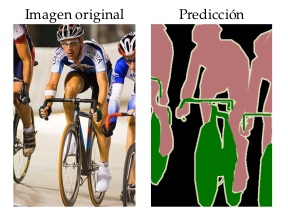
\includegraphics[width=6.5cm]{./Graphics/semseg.png}
	\caption{Resultado de una segmentación basada en píxeles. Cada color en la predicción representa una clase distinta.}
	\label{fig:semseg}
\end{figure}

\begin{property}
	Luego de la clasificación a nivel de píxeles sobre una imagen $I_{h \times w}$ a cada píxel $p_{i, j} \in I_{h \times w}$ le corresponde una única clase $w_k \in W: k \in \mathbb{N}^+$ y $W$ es un conjunto finito de clases predefinidas.
\end{property}

\subsection{Evaluación de la segmentación}

Para conocer la calidad de los resultados de un proceso de segmentación de imagen, es necesario utilizar alguna medida de evaluación. Existen diferentes medidas para lograr este objetivo. A continuación se presentan los conceptos principales para la evaluación de la calidad de los algoritmos de segmentación.

La segmentación semántica particiona los píxeles en clases, por tanto se puede resumir esta tarea a un problema de clasificación. Para evaluar clasificaciones suele utilizarse el concepto de matriz de confusión.

\begin{definition}
	Se entiende por Matriz de Confusión como una matriz bidimensional que cuantifica la frecuencia que cada categoría es bien clasificada o no frente a las otras categorías.
\end{definition}

En el caso de la clasificación binaria la matriz de confusión queda como sigue:

\begin{table}[h]
	
	\begin{tabular}{|| c || c | c ||}
		\hhline{|=||=|=|}
		
		Real /Predicción & 0 & 1\\ \hhline{||=||=|=||}
		0 & VN & FP\\
		1 & FN & VP \\ \hhline{|=||=|=|}
	\end{tabular}
\end{table}

\begin{itemize}
	\item VN representa la cantidad  de los verdaderos negativos: aquellos elementos que pertenecen a la categoría 0 y se predice que pertenecen a la categoría 0.
	\item FP representa la cantidad  de  los falsos positivos: aquellos elementos que pertenecen a la categoría 0 y se predice que pertenecen a la categoría 1.
	\item FN representa la cantidad  de  los falsos negativos: aquellos elementos que pertenecen a la categoría 1 y se predice que pertenecen a la categoría 0.
	\item VP representa la cantidad  de  los verdaderos positivos: aquellos elementos que pertenecen a la categoría 1 y se predice que pertenecen a la categoría 1.
\end{itemize}

Entre las métricas de evaluación más comunes en problemas de clasificación se encuentra:

\begin{definition}
	Precisión (P): medida que cuantifica la fracción de elementos positivos o de categoría 1 que son clasificados correctamente. 
	
	$$ P = \frac{VP}{FP + VP}$$	
\end{definition}

\begin{definition}
	Recobrado o recall (R): medida que cuantifica la fracción de elementos positivos o de categoría 1 que son clasificados.
	
	$$ P = \frac{VP}{FN + VP}$$	
\end{definition}

Estas dos medidas son de vital importancia pero por separado no indican la buena o mala calidad de los resultados en la segmentación semántca. En la segmentación no solo interesa cuan precisa es la salida del proceso sino que también se clasifique la mayor cantidad de elementos de la clase o de categoría 1. Una solución sería clasificar todos los elementos como de categoría 1, lo cual no es una respuesta factible. Por tanto se necesita un equilibrio entre ambas métricas, para lograr un recobrado alto tolerando una pequeña cantidad de falsos positivos.

A continuación se presentan dos de las medidas más utilizadas para evaluar la tarea de segmentación.

\begin{itemize}
	\item \textbf{Índice de similaridad Jaccard (IJ)}: es una métrica que permite cuantificar el solapamiento entre una máscara objetivo y la salida de algún método de segmentación. IJ cuenta el número de píxeles comunes entre la máscara objetivo y la predicción, dividido por el total de números de píxeles entre las dos máscaras.
	
	\begin{equation}
		\text{IJ} = \frac{VP}{FN + VP + FP}
	\end{equation}

	donde $GT$ es medida de verdad o \textit{ground truth}, y $P$ es la predicción.
	
	\item \textbf{Índice de similaridad de Dice (F1-Score):} es una medida que armoniza la Precisión y el Recobrado de los resultados de la segmentación. F1-Score toma un valor alto cuando P y R tiene valores altos, por lo que la determinación del valor máximo para F1-Score puede interpretarse como un esfuerzo por encontrar el mejor compromiso entre P y R.
	
		
	\begin{equation}
		\text{F1-Score} = \frac{2PR}{P + R}
	\end{equation}
\end{itemize}

\section{Reconstrucción 3D a través de Cámaras de profundidad  (RGB-D)}\label{section:rec3d}

La \textit{Reconstrucción 3D} es el proceso de generar un modelo computacional de tres dimensiones en forma de malla poligonal que refleja la apariencia y forma de una escena real con datos capturados por sensores. Una de las fuentes adquisitivas de estos datos son los sensores RGB-D integrados a las cámaras de profundidad.

Desde sus inicios el potencial de las cámaras RGB-D fue rápidamente reconocido en el campo de la visión computacional. No solo están disponibles a un bajo precio, además sus sensores capturan imágenes de color y profundidad. Dichas características las posicionan incluso por encima de costosos sistemas de escaneo 3D en determinadas tareas.

En el ámbito de la reconstrucción 3D se han diseñado numerosos e innovadores algoritmos a partir de los cuales se obtienen modelos computacionales que representan escenas estáticas, dinámicas y otros que incluso capturan propiedades adicionales. Esta tarea se puede realizar de dos formas:

\begin{itemize}
	\item Tiempo Real: donde se reconstruye  a medida que se capturan las imágenes
	\item A posteriori: donde se adquiere primeramente el conjunto de imágenes y luego se pasa al proceso de reconstrucción.
\end{itemize}

Es importante tener en cuenta estos aspectos para seleccionar el algoritmo que mejor se adecúe a la situación y condiciones ambientales del problema en cuestión. En la Figura \ref{fig:r3d} se muestra el flujo de procesamiento típico de un sistema de reconstrucción RGB-D para este tipo de escenarios.

\begin{figure}[h]
	\centering
	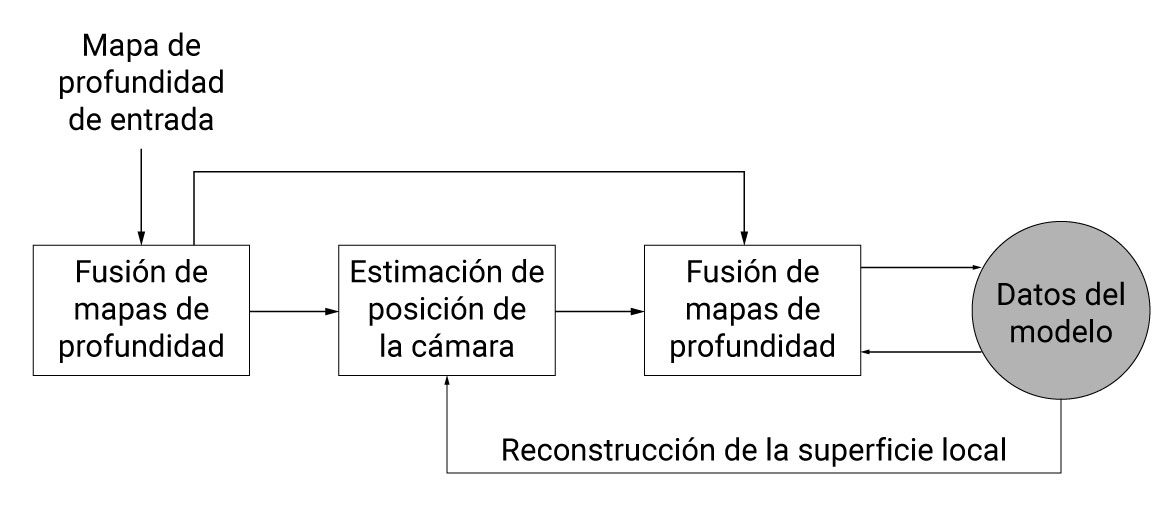
\includegraphics[width=10cm]{./Graphics/r3d.png}
	\caption{Muestra del flujo típico de un sistema de reconstrucción RGB-D: primero, la imagen de entrada preprocesada se alinea respecto a la superfice de reconstrucción actual; segundo, dada la estimación de la posición de la cámara, la entrada es integrada/fusionada en el actual modelo 3D de la reconstrucción~\cite{zollhofer2018state}.}
	\label{fig:r3d}
\end{figure}

En la próxima subsección se profundiza en un Sistema de Reconstrucción 3D a posteriori, que consecuentemente captura solo la naturalez de escenas estáticas. Por otra parte, permite realizar optimizaciones que no son factibles de ejecutar en tiempo real y puede resultar en mayor precisión de las estimaciones. Antes se presentan algunas definiciones necesarias para su comprensión.

\begin{definition}
	El Registro o Alineación entre dos imágenes (entre dos nubes de puntos) $P_1$ y $P_2$ es el proceso de encontrar una transformación espacial $M$, que minimice cierta función de distancia definida entre $P_1$ y $P_2$.
\end{definition}

\begin{definition}
	La Odometría Visual se define como el conjunto de algoritmos que ayudan a estimar el movimiento, tomando información de las imágenes capturadas por sensores.
\end{definition}

\begin{definition}
	La Función Signada de Distancia Truncada (TSDF, por sus siglas en inglés, de Truncated Signed Distance Function) es una representación volumétrica 3D de una escena donde a cada voxel~\footnote{Voxel, unidad de información gráfica que define un punto en un espacio de tres dimensiones.} almacena la distancia a la superficie más cercana~\cite{curless1996volumetric}
\end{definition}


\begin{definition}
	Malla Poligonal es una estructura de datos que consta de una colección de vértices, caras y aristas. Es utilizada para describir objetos u escenas mediante modelos poliédicos 3D. Las caras usualmente consisten en triángulos (mallas trianguales), aunque es un factor que puede variar.
\end{definition}


\subsection{Método de Reconstrucción 3D}

El flujo de trabajo descrito en esta subsección es un sistema de reconstrucción de escenas completas, basado en el artículo~\cite{choi2015robust} y adoptando ideas introducidas en~\cite{park2017colored} para lograr mejores resultados. Fue desarrollado por el equipo de la biblioteca \textit{Open3D}~\cite{zhou2018open3d}, haciendo uso de múltiples algoritmos implementados en la misma. Toma como entrada la secuencia $\hat{S}$ de imágenes RGB-D sincronizadas y alineadas, junto a la matriz intrínseca de la cámara, la cual forma parte de los parámetros entrantes de muchos algoritmos internos del sistema. Procede de la siguiente forma:

\begin{enumerate}
	\item \textbf{Construcción de Fragmentos}
	
	Las imágenes individuales tienen ruido y son incompletas. Por tanto, para manejar información más confiable de las superficies geométricas locales, se divide $\hat{S}$ en segmentos de $k$-cuadros (\textit{$k$-frames}). A todos los pares que se forman en una subsecuencia se les aplica Odometría RGB-D para estimar su alineación o registro. Se crea un grafo de posiciones de todas las imágenes del rfagmentos cuyos nodos representan una imagen RGB-D  y su posición (la primera aproximación de esta posición es la correspondiente a la alineación con su imagen antecedente en la secuencia), que transforma la geometría al espacio global del fragmento; las aristas contienen la información de la odometría entre los pares con registro satisfactorio. A las posiciones del grafo se les aplica optimización con el algoritmo Levenberg-Marquardt. Por último, cada secuencia se integra en un volumen TSDF. La malla que se extrae de cada volumen representa un fragmento a colores.
	
	\item \textbf{Registro Geométrico}
	
	Una vez creados los fragmentos de la escena el próximo paso es alinearlos en un espacio global. Primeramente, se registran los pares de  fragmentos para estimar un alianeación básica. Si son vecinos se utiliza el método ICP y en otro caso RANSAC (\textit{RANdom SAmple Consensus}) o Registro Global Rápido. Se procede a construir el grafo de posiciones de los fragmentos y se le aplica el mismo método de optimización del paso anterior.
	
	\item \textbf{Refinamiento del Registro e Integración de la Escena}
	
	Para lograr un refinamiento de las alineaciones se aplica el algoritmo ICP sobre los pares detectados en registro geométrico; se crea un nuevo grafo de posiciones con los registros refinados; y se ejecuta la optimización en dichas posiciones como previamente mencionado en 1. El último paso del sistema es la integración de todas las imágenes RGB-D en un solo volumen TSDF y la extracción de la malla resultante.
\end{enumerate}

\begin{figure}[h]
	\centering
	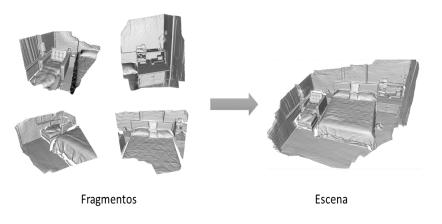
\includegraphics[width=10cm]{./Graphics/algo3d.png}
	\caption{Ejemplo de resultados del algoritmo de reconstrucción. A la derecha se muestra el conjunto de fragmentos de la escena y a la izquierda la reconstrucción final formada a partir de los fragmentos. El ejemplo muestra la escena sin colores.}
\end{figure}

\section{Estimadores de perímetro, área y volumen en mallas poligonales}\label{section:measure}

El diseño de estimadores espaciales como son el perímetro, área y volumen en mallas poligonales constituye otra de las tareas trascendentales del trabajo. 

DEFINICION DE CONVEX HULL

\subsection{Perímetro}

El perímetro de una malla poligonal que representa una úlcera se define como la longitud de los lados de la figura en 2D de la úlcera. Para la estimación del perímetro se procede:

\begin{enumerate}
	\item \textbf{Proyección al plano}
	
	Se concibe como la etapa en la que se proyecta la malla poligonal en tres dimensiones en una figura plana. La nube de puntos $P$ que conforma la malla está compuesta por puntos de tres componentes $p_i = (x_i, y_i, z_i)$. Para la proyección se transforma la nube de puntos $P$ en $P_{2D}$ la cual cumple que $\forall p_i \in P_{2D}: p_i = (x_i, y_i, 0)$.
	
	\item \textbf{Envoltura convexa de $P_{2D}$}
	
	Los puntos $p_{qhull}$ se definen como los vértices de la envoltura convexa de $P_{2D}$. Se calcula la envoltura convexa de $P_{2D}$ y se toman los $p_{qhull}$ y las aristas.
	
	\item \textbf{Sumatoria de la distancia entre puntos $p_{qhull}$}
	
	Luego, el perímetro total de la úlcera no es más que la suma de la longitud de las aristas o la distancia entre los $p_{qhull}$ adyacentes. Para calcular la longitud se utiliza la distancia euclideana.
	
\end{enumerate}

\subsection{Área}

MUELA DEL AREA

La estimación del área de una malla poligonal se define como la sumatoria del área de todas las caras triangulares que conforman la malla. Para el cálculo del área de los triángulos se utiliza la fórmula de Herón. 

$$A = \sqrt{s(s-a)(s-b)(s-c)}$$

donde $s = \frac{P_t}{2}$ y $P_t$ es el perímetro de la cara triangular. Por tanto, el área de la malla poligonal $A_M$ con $k$ caras se calcula como:

\begin{equation}
	A_M = \sum_{i = 0}^{k} A_k
\end{equation}

donde $A_k$ es el área de la cara $k$-ésima de la malla poligonal.

\subsection{Volumen}

MUELA DEL VOLUMEN

La estimación del volumen de una úlcera en este caso particular se concibe como un proceso de varias etapas. Las úlceras se pueden definir como cavidades en una superficie, por tanto el volumen de una úlcera no es más que el volumen de la cavidad. Luego es necesario aproximar la superficie que cubre la cavidad, esta superficie será llamada tapa $T_U$ de la úlcera con malla $U$. Luego, se forma la malla compuesta de $C = T_U + U$ y se calcula el volumen de esta malla, realizando una triangulación de Delaunay y sumando el volumen de las pirámides resultantes.



\chapter{Sistema de medición 3D}\label{chapter:proposal}

El flujo de trabajo del sistema desarrollado consta de 5 etapas: la captura de las imágenes RGB-D, seguimiento de la zona de la úlcera seleccionada de forma asistida, la segmentación, la reconstrucción 3D y las mediciones.

\section{Captura}

Uno de los objetivos fundamentales es la elaboración de un sistema de bajo costo. En el mercado existen diversas cámaras RGB-D con distintas resoluciones y características. La cámara utilizada en este trabajo es la Intel\textregistered~RealSense\texttrademark~D435i, pues es una cámara de costo justo para su precisión y calidad.

\begin{figure}[ht]
	\centering
	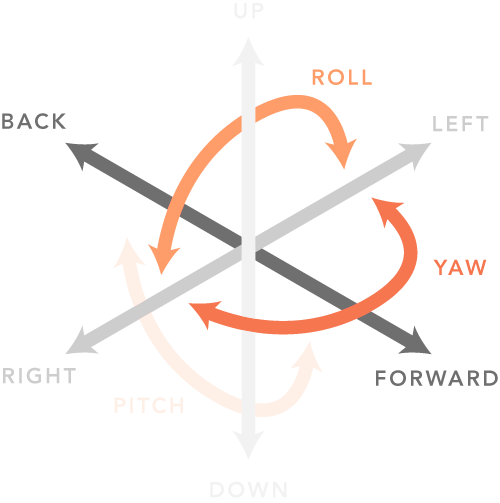
\includegraphics[width=4cm]{./Graphics/6dof.png}
	\caption{Los 6 grados de libertad en la IMU de la Intel\textregistered~RealSense\texttrademark~D435i.}
	\label{fig:6dof}
\end{figure}

El dispositivo al ser una cámara de profundidad estéreo, cuenta con dos cámaras RGB de resolución 1920 $\times$ 1080 píxeles, con un \textit{baseline} de $5,5$ cm y un sensor de láser infrarrojo que mejora la habilidad del sistema estéreo de medir profundidad. Además, cuenta de una unidad inercial (IMU, por sus siglas en inglés) que permite cuantificar el movimiento del dispositivo. El módulo IMU es de 6 grados de libertad que señala la libertad de movimiento de un cuerpo rígido en el espacio tridimensional: (1) hacia adelante/hacia atrás, (2) arriba/abajo, (3) izquierda/derecha (estos se refieren a traslaciones respecto a los ejes coordenados), además (4) cabeceo o \textit{pitch}, (5) guiñada o \textit{yaw}, y (6) alabeo o \textit{roll} (que denotan rotaciones con los ejes coordenados como eje de rotación) (Figura \ref{fig:6dof}). En la Tabla \ref{tab:d435i} se muestran las características principales de la cámara.

\setlength{\tabcolsep}{0.5em} % for the horizontal padding
{\renewcommand{\arraystretch}{1.2}% for the vertical padding
\begin{table}[ht]
	\centering
	\begin{tabular}{lll} 
		\hhline{===}
		& \multicolumn{2}{l}{\textit{Intel\textregistered~RealSense\texttrademark~D435i}}  \\ 
		\hhline{===}
		\multirow{2}{*}{Cámara RGB}                     & Resolución & 1920 $\times$ 1080 px                                       \\ 
		\cline{2-3}
		& fps        & 30 fps                                       \\ 
		\hline
		\multirow{2}{*}{Cámara IR}                      & Resolución &     1280 $\times$ 720 px                                   \\ 
		\cline{2-3}
		& fps        & 30 fps                                    \\ 
		\hline
		Rango                                           &            & $0.2\sim3$ metros                                \\ 
		\hline
		Sensor                                          &            & Cámara estéreo                                \\ 
		\hline
		\multirow{2}{*}{Campo de visión del sensor RGB} & Horizontal          & $91.2^\circ$                                       \\ 
		\cline{2-3}
		& Vertical         & $65.5^\circ$                                       \\ 
		\hline
		\multirow{2}{*}{Campo de visión del sensor IR}                    & Horizontal         & $90^\circ  \pm 3^\circ$                                     \\
		\cline{2-3}
		& Vertical         & $63^\circ  \pm 3^\circ$                                 \\ 
		\hline
		Conector USB                                             &            & USB 2.0/ USB 3.1 Gen 1                                    \\
		\hline
		Unidad de Medición Inercial & & 6 grados de libertad
		\\
		\hline
	\end{tabular}

	\caption{Propiedades de la cámara Intel\textregistered~RealSense\texttrademark~D435i} 
	\label{tab:d435i}
\end{table}

La captura de muestras se efectuó en un ambiente no controlado, en las consultas y salones de curas del Instituto Nacional de Angiología y Cirugía Cardiovascular (INACV). Durante el proceso de captura se sostiene y se mueve la cámara alrededor de la zona de interés para la toma de la secuencia. Es necesario colocarla a una distancia de la UPD de aproximadamente 20-25 centímetros. Para los posteriores procesos es requerida la alineación y sincronización de cada uno de los pares de imágenes de profundidad y RGB.  Los detalles y estadísticas de las muestras obtenidas en el centro hospitalario se presentan en la Sección \ref{sec:dataset}.

En las consultas los médicos suelen utilizar paños de color verde para cubrir las zonas que no son de interés. Estos paños añaden información indeseada en el proceso de segmentación, por tanto, se decidió eliminar el mismo de forma automática, utilizando segmentación basada en la aplicación de umbral de colores. Se cambia el espacio de color de las imágenes RGB a HSV y los píxeles que sus valores en el espacio nuevo se encuentren entre $[25, 52, 72]$ y $[102, 255, 255]$, se sustituyen por color blanco $[255, 255, 255]$. Para esto se construye una máscara y se aplica el operador morfológico abierto para luego hacer la sustitución de color en la imagen RGB de entrada (Figura \ref{fig:tissue}).

\begin{figure}[ht]
	\centering
	\begin{subfigure}
		\centering
		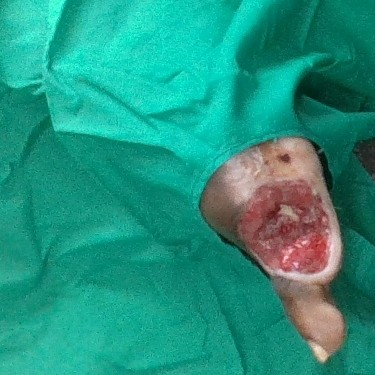
\includegraphics[width=.2\linewidth]{./Graphics/a.jpg}
	\end{subfigure}
	\begin{subfigure}
		\centering
		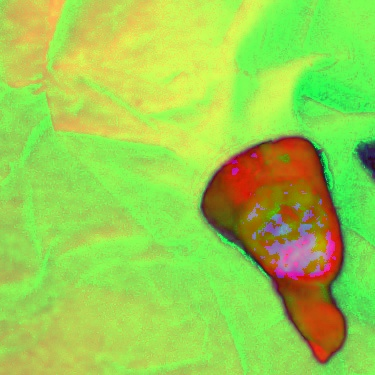
\includegraphics[width=.2\linewidth]{./Graphics/hsv.jpg}
	\end{subfigure}
	\begin{subfigure}
		\centering
		
\includegraphics[width=.2\linewidth]{./Graphics/tissue-mask.jpg}
	\end{subfigure}
	\begin{subfigure}
		\centering
		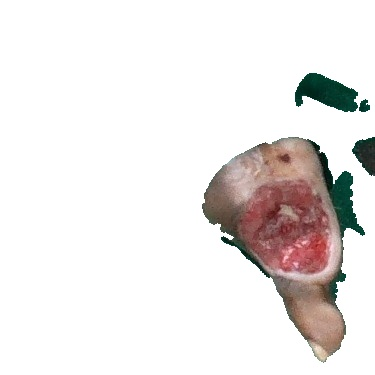
\includegraphics[width=.2\linewidth]{./Graphics/res.jpg}
	\end{subfigure}
	\caption{Proceso de segmentación del pañuelo para su eliminación automática: (1) se toma la imagen en RGB, (2) se convierte a HSV, (3) se seleccionan los píxeles por el umbral y (4) se aplica la máscara a la imagen en RGB.}
	\label{fig:tissue}
\end{figure}

Las imágenes RGB al ser obtenidas en un ambiente sin control de la iluminación y el enfoque pueden carecer del contraste suficiente o presentar ruido de emborronamiento (motion blur) producto del movimiento de la cámara. Por tales razones, se propone después de la etapa de captura aplicar el filtro de \textit{sharpening} y el mejoramiento de contraste usando el algoritmo CLAHE.



\section{Seguimiento de la zona de la UPD seleccionada de forma asistida}\label{segasis}

Las imágenes capturadas en el proceso anterior contienen demasiada información innecesaria para el algoritmo de segmentación propuesto por lo que se aumenta el umbral de error en la predicción. En las imágenes se captura la úlcera además de otros objetos presentes en el entorno pero que no son de interés para el algoritmo como son: herramientas de trabajo, el piso, utensilios y equipos médicos, entre otros. Por tal razón, se decidió adoptar un enfoque asistido para una pre-segmentación. 

El enfoque asistido consiste en que el especialista que captura la muestra centrará la atención del sistema en un área específica reduciendo el nivel de ruido e información excedente. El especialista que realiza la captura enmarcará la zona donde se encuentra la úlcera marcando mediante un rectángulo (o cuadrado) una zona de la imagen en cuyo centro se encuentra aproximadamente la UPD. Se utiliza el algoritmo de seguimiento de objetos en vídeo descrito en la Sección \ref{sec:csr} conocido como CSR-DCF. Con este enfoque se consigue una posición del cuadrado donde se encuentra la úlcera en cada cuadro o \textit{frame} de la muestra de vídeo. Estas subimágenes son las que se utilizan como entrada al algoritmo de segmentación.

\section{Segmentación}

En los procedimientos descritos en~\cite{wang2014smartphone, filko2018wound}, la segmentación de la UPD se ejecuta independiente y posterior a la reconstrucción 3D. Sin embargo, en este proyecto se trata desde otra perspectiva, que consiste en segmentar todas las imágenes RGB obtenidas en la captura para luego realizar la reconstrucción a partir de las máscaras que se obtienen. Al reconstruir utilizando las imágenes RGB luego de aplicar las máscara binaria, se logra una superficie de la escena donde solo tienen color las zonas de la úlcera, y el resto de los puntos aparecen en negro, luego estos puntos se eliminan para proceder a medir la malla.

Por tanto, el primer paso es ejecutar una segmentación de las imágenes RGB capturadas y recortadas por CSR-DCF. De cada una se obtiene una máscara, donde la zona de la lesión se exhibe en blanco y el resto en negro (Figura \ref{fig:dfuseg}). Estas imágenes junto con las originales RGB-D serán utilizadas en la reconstrucción para crear el modelo 3D sobre el cual se realizarán mediciones.

\begin{figure}[ht]
	\centering
	\begin{subfigure}
		\centering
		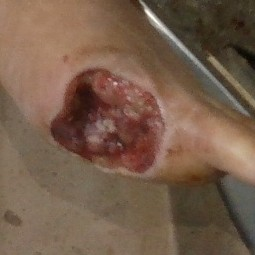
\includegraphics[width=.3\linewidth]{./Graphics/dfu.jpg}
	\end{subfigure}
	\begin{subfigure}
		\centering
		
\includegraphics[width=.3\linewidth]{./Graphics/mask.jpg}
	\end{subfigure}
	\caption{Imágenes RGB de las úlceras y las máscaras de segmentación}
	\label{fig:dfuseg}
\end{figure}

La segmentación de las imágenes RGB puede ser lograda utilizando métodos tradicionales, como se explica en el capítulo \ref{chapter:state-of-the-art}. Sin embargo, estos están limitados por sus capacidades para la descripción de las características de las heridas. En la última década el Apredizaje Profundo ha adquirido popularidad en este ámbito. Toma ventaja de la poderosa habilidad de extracción de características de entrenadas Redes neuronales profundas (Deep Neural Networks, DNN) para el procesamiento de imágenes. Una desventaja es que requieren de grandes cantidades de datos durante el proceso de aprendizaje.

La redes neuronales UNet y LinkNet, descritas en la Sección \ref{sec:nn} del capítulo \ref{chapter:theoretical-framework}, son conocidas por sus buenos resultados en la tarea de segmentación de imágenes biomédicas y sin sacrificar el tiempo de procesamiento. En los artículos~\cite{chino2020segmenting, cui2019diabetic} se hace uso de las mismas para la segmentación de UPD y se muestran comparaciones con otros trabajos, respecto a los cuales se observan mejoras. Apoyándose en la generación de nuevas imágenes y en su arquitectura, brindan una alternativa favorable para el entrenamiento con pocos datos anotados. 

En el artículo~\cite{mahbod2021automatic} se propone emplear un conjunto de estas redes neuronales prediciendo en \textit{average ensemble}~\footnote{se dice de aquel predictor que su resultado depende del promedio de predictores anteriores.}. Se utilizan modelos pre-entrenados en los caminos de expansión en ambas arquitecturas. En el caso de la arquitectura UNet se utilizan los pesos del modelo EfficientNetB2~\cite{tan2019efficientnet} y en la arquitectura LinkNet se utilizan los pesos del modelo EfficientNetB1~\cite{tan2019efficientnet}, ambos modelos son pre-entrenados en el conjunto de datos Medetec~\cite{medetec}. En ese entrenamiento se utilizó la técnica de Aumento de Datos conocida como \textit{Data Augmentation} aplicando rotaciones y \textit{flips} en varios sentidos para obtener nuevas imágenes. En lugar de entrenar todas las redes sobre Medetec, se dividió el conjunto de datos en 5 subgrupos y se entrenó una red de cada arquitectura en cada uno de los subgrupos. Durante el proceso de predicción cada imagen pasa por cada uno de las 10 redes entrenadas y se obtienen 10 máscaras de segmentación semántica, luego se utiliza el promedio de las máscaras como predicción final. Luego de que se obtiene la máscara de segmentación se obtiene la imagen binaria de la misma y se le aplica un posprocesamiento, en el que se remueven los objetos bien pequeños y se rellenan los agujeros, aplicando la operación cerrado de morfología (Figura \ref{fig:pipeSeg}).

\begin{figure}[ht]
	\centering
	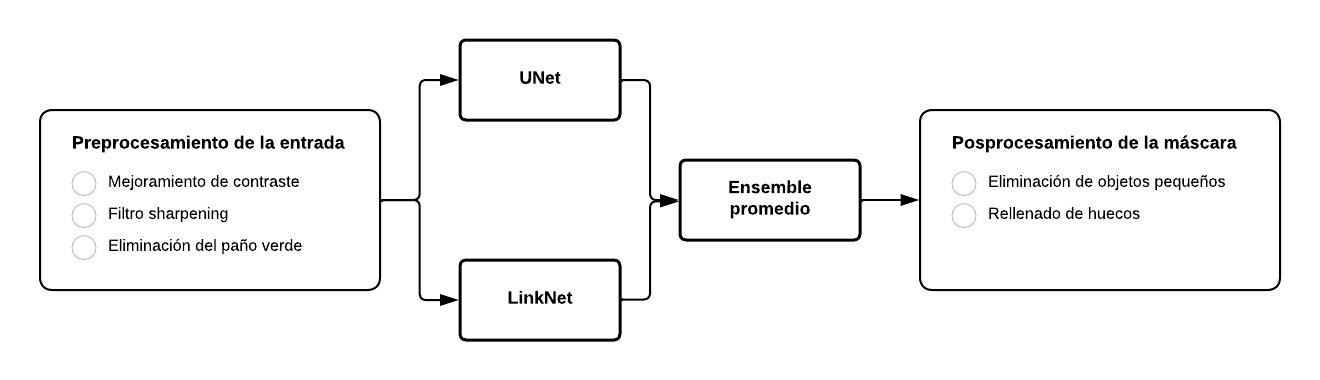
\includegraphics[width=12cm]{./Graphics/segmentation.png}
	\caption{Diagrama del algoritmo de segmentación propuesto}
	\label{fig:pipeSeg}
\end{figure}

\section{Reconstrucción 3D}

Para el proceso de reconstrucción 3D se plantea el uso del marco de trabajo (framework) \textit{Open3D}~\cite{zhou2018open3d}, una biblioteca de código abierto que expone un conjunto de estructuras de datos y algoritmos tanto en C++ como en Python. El \textit{back-end} está altamente optimizado y está configurado para la paralelización.

En \textit{Open3D} se proponen dos flujos de trabajo para la reconstrucción que se explican a continuación:

\begin{itemize}
	\item Basado en~\cite{dong2022ash} se formula un método en tiempo real u \textit{online}. Este realiza la reconstrucción volumétrica y un SLAM~\footnote{del inglés \textit{Simultaneous Localization and Mapping}} denso usando tensores y la interfaz de \textit{Hash Map} del propio \textit{Open3D}~\footnote{\textit{Open3D} permite paralelizar el \textit{hashing} tanto en la Unidad Gráfica de Procesamiento (GPU, por sus siglas en inglés) como en la Unidad Central de Procesamiento (CPU) usando llaves y valores organizados como tensores, donde se toma un lote de llave y/o valor como entrada}.
	\item Una reconstrucción a posterior u \textit{offline} completa de la escena a partir de una secuencia RGB-D. Esta está basada en~\cite{choi2015robust} y las ideas introducidas en~\cite{park2017colored} para una mejor reconstrucción.
\end{itemize}

A diferencia de los sistemas de reconstrucción en tiempo real, que no admiten alta complejidad, los \textit{offline} permiten el uso de algoritmos más complejos y demandantes desde el punto de vista computacional. Al no contar en esta propuesta con cámaras de una alta resolución (costo muy elevado) se pueden presentar errores de precisión.  Esto, sumado a la naturaleza estática de la escena, lleva a que un sistema de reconstrucción 3D \textit{offline} brinde mejoras en la calidad de los modelos 3D finales. 

En la Sección \ref{section:rec3dmet} se describe el funcionamiento de este sistema. La entrada consiste en la matriz intrínseca junto con la secuencia de imágenes RGB-D a reconstruir. La matriz se construye con los parámetros intrínsecos de la cámara, calculados mediante el proceso de auto-calibración descrito en la sección \ref{section:calibration}. Para alinear las imágenes de color con las de profundidad se realiza una transformación geométrica por píxel en función de los datos de profundidad proporcionados. 

Con estos datos de entrada el sistema estima la posición de cada imagen RGB-D en el espacio global; posteriormente, se integran en un solo volumen TSDF que brinda como resultado un modelo 3D que describe la escena, representado a través de una malla poligonal a colores.

\begin{figure}[ht]
	\centering
	\begin{subfigure}
		\centering
		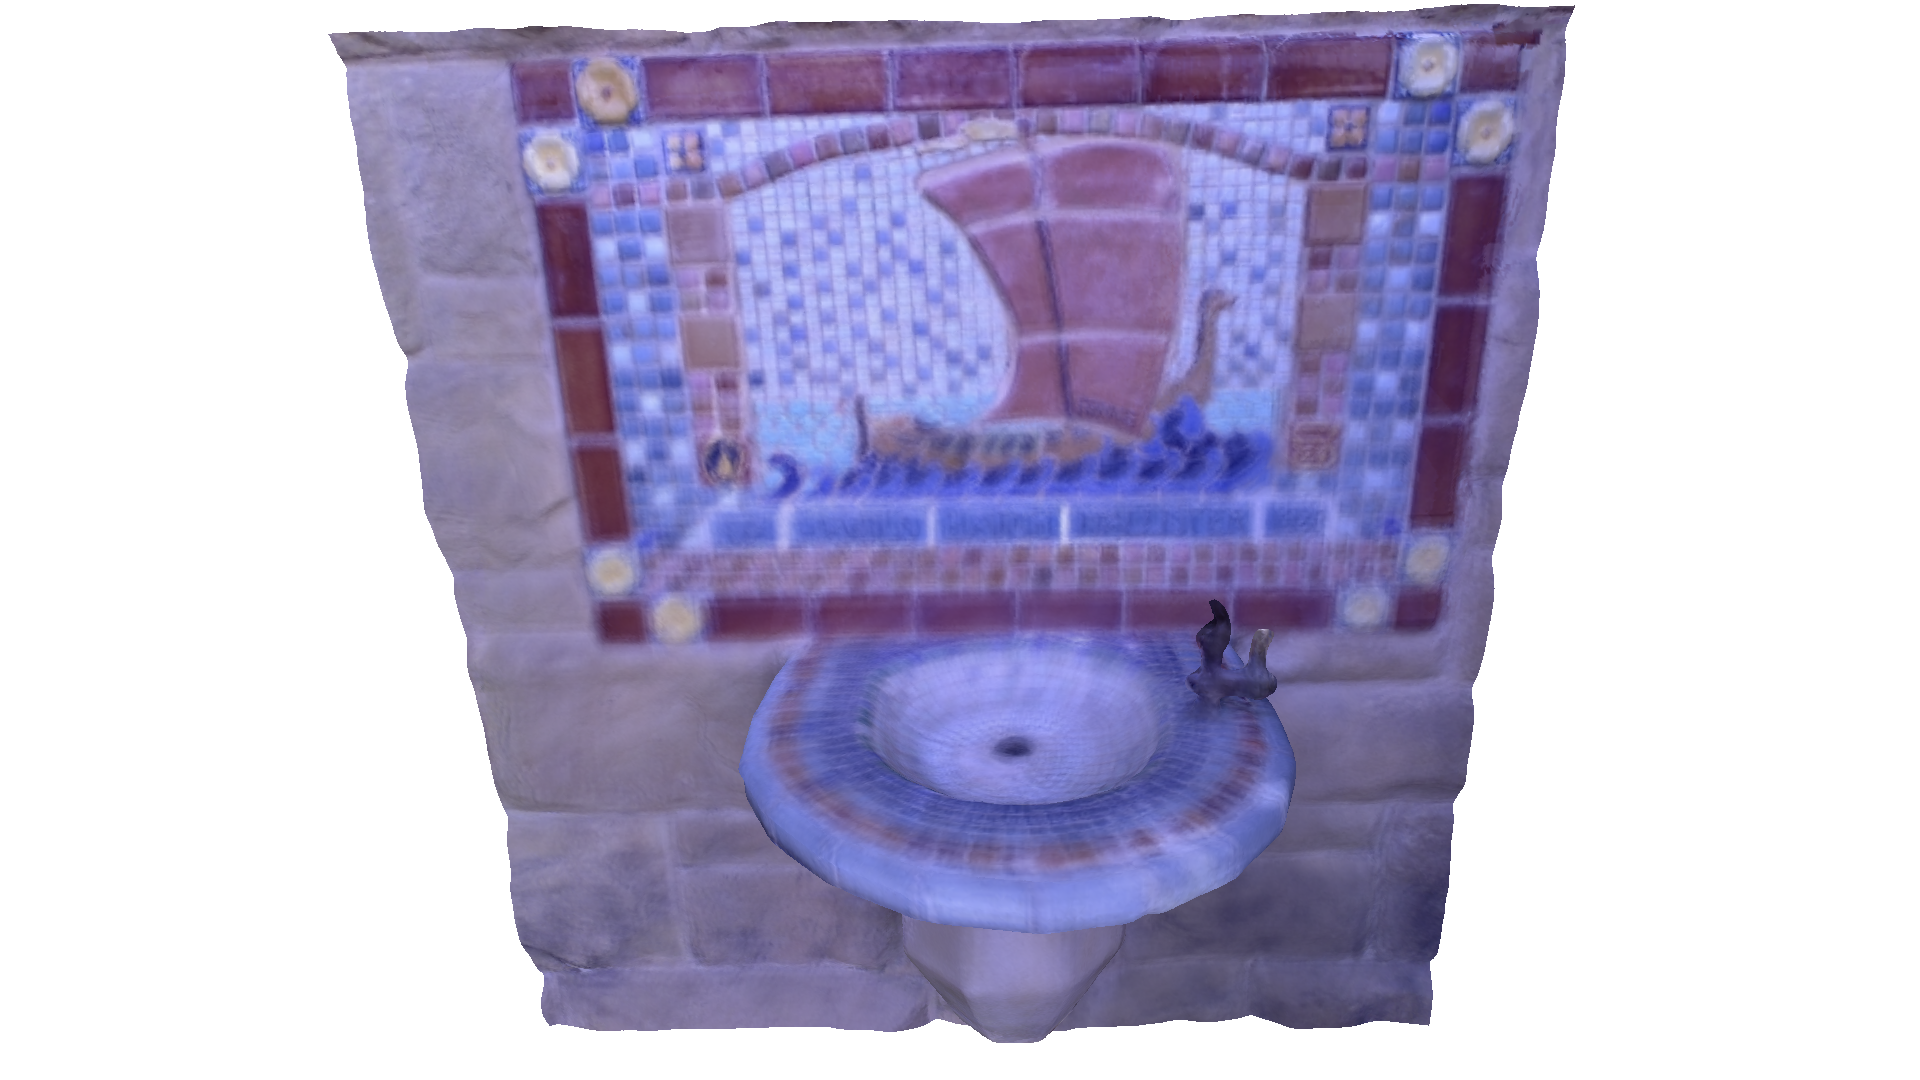
\includegraphics[width=.4\linewidth]{./Graphics/co1.png}
	\end{subfigure}
	\begin{subfigure}
		\centering
		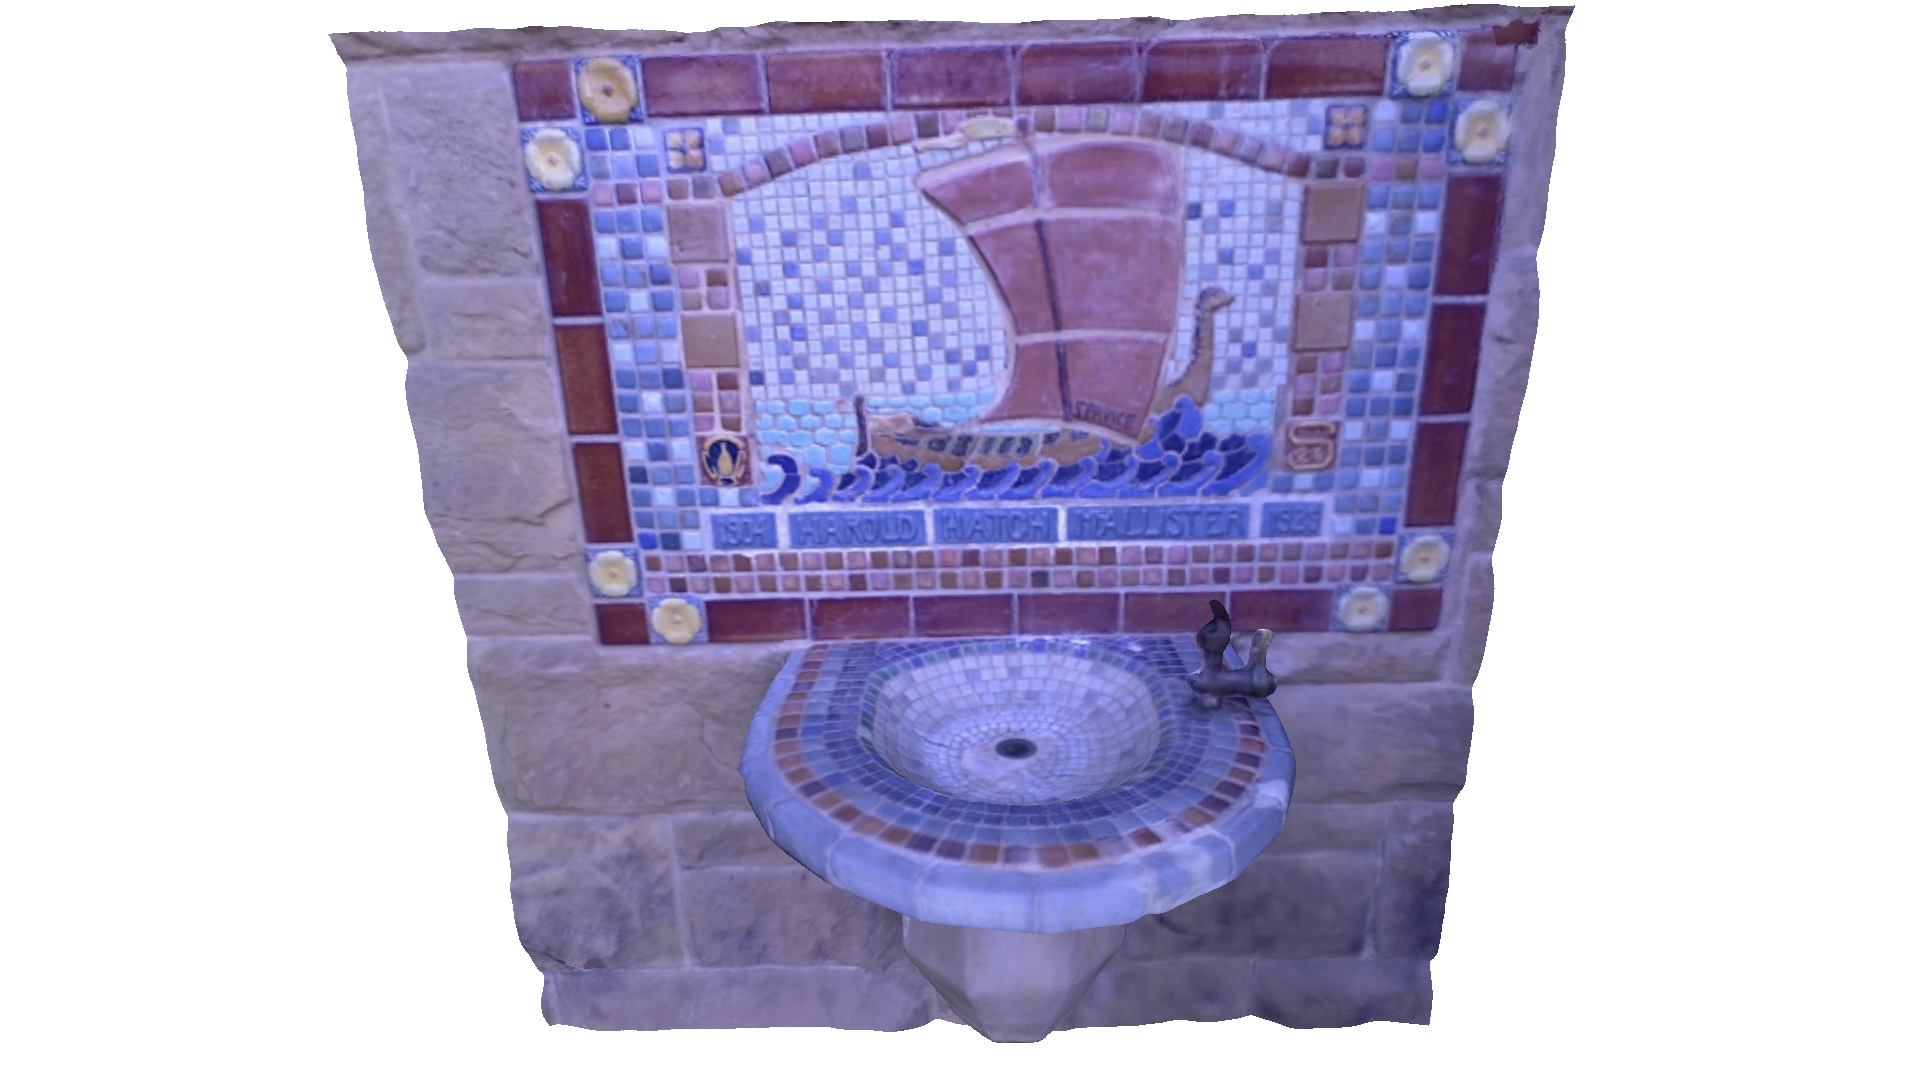
\includegraphics[width=.4\linewidth]{./Graphics/co2.png}
	\end{subfigure}
	\caption{Resultado del método de optimización de mapas de color propuesto en~\cite{zhou2014color}.}
	\label{fig:optColor3d}
\end{figure}

Dado que los marcos de color y profundidad no están perfectamente alineados si se hacen corresponder los colores a la geometría reconstruida la correspondencia de texturas puede resultar en un mapa de color borroso (Figura \ref{fig:optColor3d}). La biblioteca \textit{Open3D} proporciona para este caso el método de optimización de mapas de color propuesto por~\cite{zhou2014color}. Pero se necesita un segundo modelo que defina la segmentación 3D. Para lograrlo se modifica el último paso de la reconstrucción, la integración de la escena. Esta vez se sustituyen las imágenes RGB por las máscaras resultantes de la segmentación 2D aplicadas a las imágenes de color y se aprovecha la estimación de la posición global obtenidas de los fragmentos registrados con las imágenes de color sin segmentar. De esta forma se adquiere una malla que solo presenta colores en la región segmentada, para luego eliminar de esta todo vértice que tenga un color negro puro y las aristas que unen a los mismos.

\section{Mediciones}

La propuesta para las mediciones utiliza los algoritmos presentados en la Sección \ref{section:measure}. Se recibe un archivo \texttt{.ply} con el modelo resultante de la reconstrucción 3D. De este modelo se extrae la nube de puntos y la malla poligonal del modelo para realizar la medición. La escala de las coordenadas de los puntos se fija en milímetros (mm) a través del parámetro \texttt{DEPTH\_UNITS} en la cámara. Este parámetro representa el número de metros por unidad de profundidad. Luego, las mediciones en el sistema se expresan en milímetros.

Para el perímetro se trabaja sobre la nube de puntos del modelo. Se construye una nube de puntos en 2D, anulando la componente de profundidad $z$. Esto con el fin de calcular la envoltura convexa en esta nueva nube de puntos, y obtener los puntos que están en la envoltura convexa, o sea, los puntos frontera. Luego, se calcula la distancia entre estos puntos. Al eliminar la componente $z$ de la nube de puntos no se afecta la precisión de la medición pues se mantiene la noción de distancia en el plano $XY$ obtenida de la reconstrucción, la cual es suficiente a la hora de estimar el perímetro.  

Para el área se trabaja con la malla poligonal del modelo, calculando el área total como la sumatoria del área de los triángulos de la malla, utilizando la fórmula de Herón. Luego, se divide el resultado entre \texttt{DEPTH\_UNITS}$^2$ para obtener el área.

Para el volumen se trabaja con la nube de puntos, se calcula la envoltura convexa de la nube de puntos y se realiza la interpolación de la tapa, y luego se realiza la triangulación de Delaunay entre la tapa y la úlcera. Posteriormente se procede a calcular el volumen total como la sumatoria del volumen de las pirámides resultantes. Luego, se divide el resultado entre \texttt{DEPTH\_UNITS}$^3$ para obtener el volumen. 


\section{Flujo de trabajo del programa}

En las secciones anteriores se han descrito los flujos de trabajo de las distintas etapas del sistema. El programa propuesto no es más que una aplicación de consola, donde se reciben los datos relativos al paciente, tales como: nombre, edad, sexo, tipo de diabetes y localización de la úlcera. Luego se procede a capturar la muestra utilizando la cámara de profundidad, asistida por el algoritmo de seguimiento o rastreo de objetos en secuencias de vídeo. Posteriormente, se obtienen las imágenes RGB de la escena, las imágenes comprendidas dentro de \textquotedblleft la caja\textquotedblright\ de seguimiento y las imágenes de profundidad de la escena. Las imágenes del interior de la caja se proveen como entrada al algoritmo de segmentación y se obtienen las máscaras correspondientes. Estas máscaras de segmentación se amplían hasta la resolución de las imágenes de la escena, se toma la región segmentada y se introduce al algoritmo de reconstrucción 3D junto a las imágenes de profundidad. La reconstrucción retorna un modelo 3D de la escena, se elimina toda la información no relacionada con la región segmentada en el modelo. Sobre este modelo segmentado se realizan las mediciones correspondientes al perímetro, el área y el volumen. Como finalización del flujo se exporta un archivo \verb|.pdf| con la información del paciente y las mediciones. 

\begin{figure}[h]
	\centering
	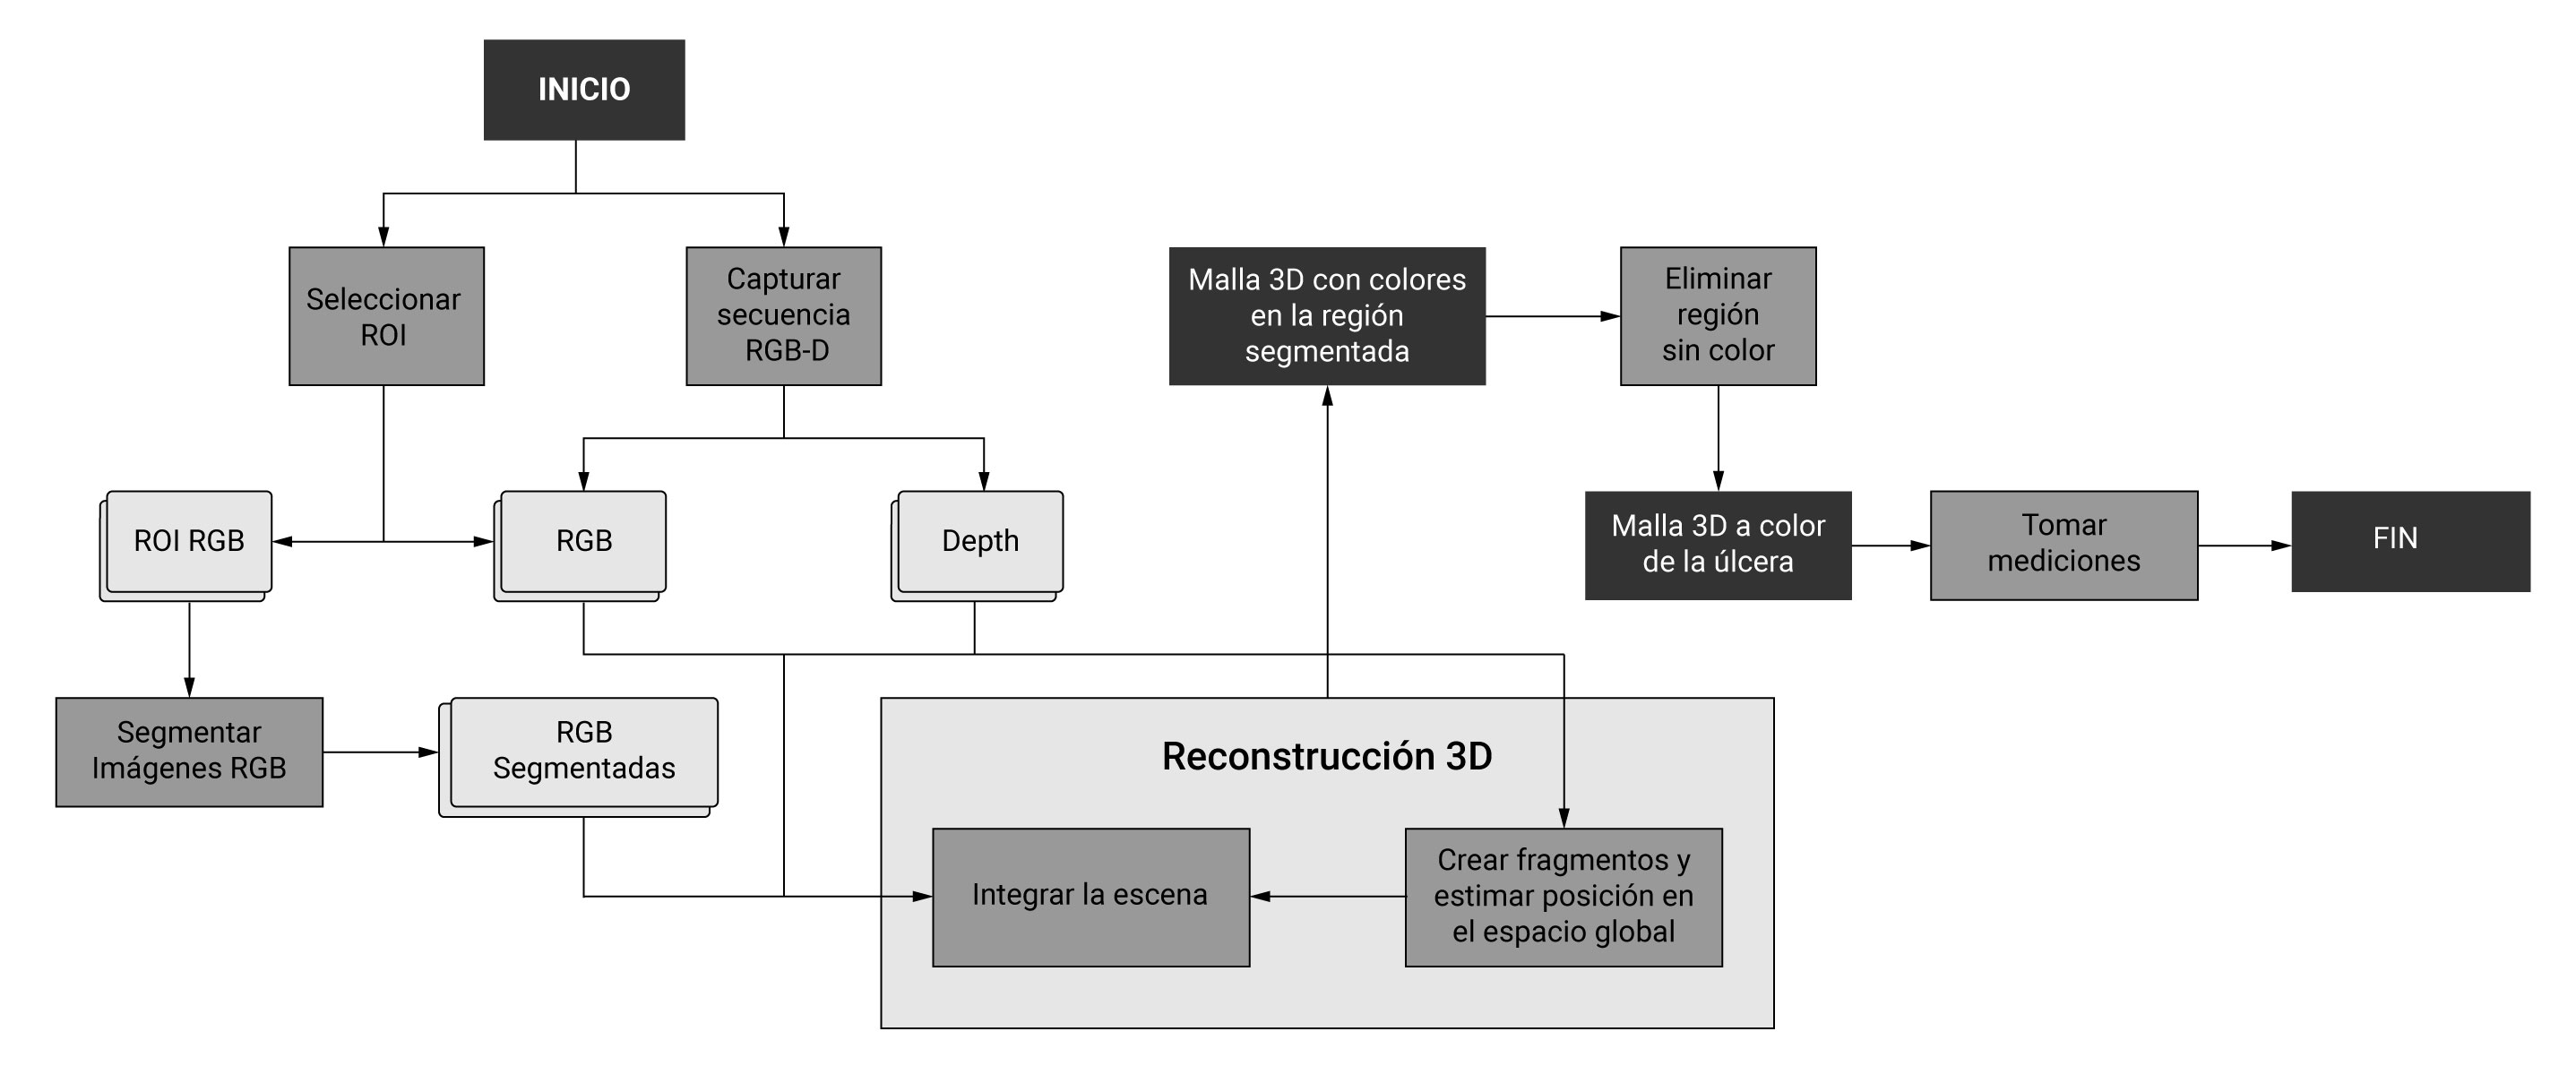
\includegraphics[width=15cm]{./Graphics/flow.jpg}
	\caption{Diagrama de flujo de la aplicación propuesta}
	\label{fig:flowCLI}
\end{figure}
\chapter{Experimentos y Detalles de Implementación}\label{chapter:implementation}

En este capítulo se presentan los experimentos realizados en la investigación para el desarrollo del sistema de segmentación, reconstrucción y medición de úlceras de pie diabético. Además, se presentan los resultados y argumentos sobre las decisiones tomadas en la propuesta final. En adición, se brindan detalles de la implementación y breves descripciones de las herramientas con que cuenta el software desarrollado.

Para el desarrollo de los experimentos se poseían dos computadoras: una de ellas con un CPU Intel\textregistered~Core\texttrademark~i5-8250U a 1.60GHz de 64-bit, con 8 Gb de RAM y con sistema operativo Ubuntu 20.04 LTS; la otra computadora con un CPU Intel\textregistered~Core\texttrademark~i7-4770HQ a 2.20GHz de 64-bit, con 16 Gb de RAM y sistema operativo MacOS 10.9.4. Además, para agilizar el procesamiento con las redes neuronales de la segmentación se contaba con la arquitectura de Google Colab con GPU NVIDIA K80. La cámara disponible era la Intel\textregistered~RealSense\texttrademark~D435i, la cual a distancias cortas provee mediciones de profundidad buenas para el desarrollo del proyecto; a diferencia de la cámara de profundidad de Microsoft \textit{Kinect v1} usada en~\cite{ching2022segm3d}, esta provee modelos 3D de calidad.

\section{Construcción del conjunto de datos}

Como seguimiento al trabajo~\cite{ching2022segm3d} se construyó un conjunto de datos que contiene secuencias de vídeo RGB-D de las úlceras de pie diabético. Las muestras se tomaron en el período de tiempo comprendido en los meses de abril a junio de 2022 en la consulta de angiología del INACV y el salón de curas de la sala ``Elpidio Sosa González'', en coordinación con los especialistas: Dr. José I. Fernández Montequín, Dr. Héctor T. Álvarez Duarte y Dr. Abraham Martínez.

En la captura de los datos era imprescindible obtener información relativa a la evolución de la UPD a lo largo del tiempo, por tal razón, se tomaron muestras de la misma úlcera con períodos de separación de mínimo una semana. Además, se obtuvieron datos relativos al paciente como nombre, edad, sexo, color de la piel, tipo de diabetes, tipo de úlcera, localización de la úlcera, así como la muestra de vídeo en RGB-D y el modelo 3D extraído con la cámara y el Intel\textregistered~RealSense\texttrademark~Viewer incluido en el SDK 2.0. Toda esta información se publica en el conjunto de datos a excepción del nombre del paciente, en su lugar se adjunta un código identificador compuesto por las iniciales del nombre, la edad y el sexo, por ejemplo: sea el paciente Susanny Vega Cintra de edad 25 años y sexo femenino, entonces su código de identificación es SVC-25-F.

El conjunto de datos está compuesto por 32 pacientes con edad promedio de 63 años; de estos pacientes, 23 de ellos son de sexo masculino y 9 de sexo femenino. Los colores de piel de los pacientes tenidos en cuenta tienen la siguiente distribución: 20 pacientes de piel blanca, 6 de piel negra, 5 de piel mestiza y 1 de piel amarilla. Los pacientes en su mayoría son diabéticos de tipo II, con una representación de 29 individuos, 2 diabéticos de tipo I, y 1 paciente que no era diabético. Se tomaron 65 muestras de úlceras de los 32 pacientes. Las úlceras estudiadas en su mayoría son úlceras de pie diabético de tipo neuro-infeccioso. La distribución del tipo de úlceras es: 20 úlceras neuro-infecciosas, 8 isquémicas, 3 flebolinfáticas y 1 lesión combinada. Las úlceras tienen mayor presencia en el pie izquierdo con un total de 22 y 10 en el pie derecho, donde las zonas con mayor afectación son los dedos, el dorsal del pie y la planta del mismo (Figura \ref{fig:loc}).

\begin{figure}[ht]
	\centering
	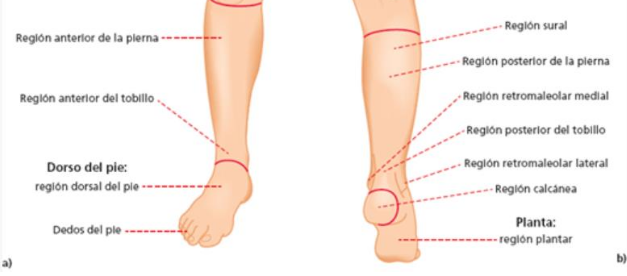
\includegraphics[width=10cm]{./Graphics/human.png}
	\caption{Las localizaciones anatómicas donde se presentan las lesiones}
	\label{fig:loc}
\end{figure}

Para la experimentación con la segmentación y la reconstrucción se tomaron 20 UPD del conjunto de datos anterior de 9 pacientes, y se extrajo un conjunto de imágenes RGB y de profundidad de las secuencias de vídeo. La extracción consistió en extraer uno de cada diez \textit{frames} del vídeo, por tal razón, se obtuvieron un total de 420 imágenes RGB y de profundidad. Todas las imágenes RGB no poseían la calidad necesaria para la experimentación, por tal razón, se hizo una eliminación manual utilizando como criterios de calidad lo siguiente:

\begin{itemize}
	\item Ausencia de ruido por movimiento o \textit{motion noise}.
	\item Iluminación adecuada en la zona de ulcerosa, en este caso, se utilizó como medición de la iluminación la perspectiva del ojo de quien realizó la eliminación. 
	\item Úlcera completamente visible. 
\end{itemize}

Las imágenes que incumplieran uno o varios de los criterios de calidad se descartaron. Luego de filtrar el conjunto con el criterio anterior se obtuvo un subconjunto de 253 imágenes. Para el proceso de segmentación era necesario obtener el \textit{ground truth} o segmentación verdadera de las imágenes. Para ello se elaboraron se forma manual un total de 135 \textit{ground truth} que fueron validadas por los especialistas. Sobre este conjunto de 135 imágenes con sus respectivos \textit{ground truth} validados se realizaron todos los procedimientos de experimentación.

\section{Experimentos e implementación de la segmentación de UPD}

Los experimentos desarrollados con el algoritmo de segmentación abarcan la evaluación de la capacidad del modelo de predecir los bordes de la úlcera en las imágenes obtenidas con las cámaras de profundidad. En caso, de reportarse un mal o ineficiente rendimiento del modelo con las nuevas imágenes se exploran técnicas de preprocesamiento, así como de asistencia al algoritmo para que se enfoque en la región de interés. Además, se exploran las razones de los fallos del algoritmo de segmentación. 

\subsection{Experimentación con el algoritmo de segmentación}

La experimentación con el algoritmo de segmentación incluye la predicción y el análisis de las métricas expuestas en la Sección \ref{sec:evalSeg}. 

El primer experimento que se desarrolló fue introducir las imágenes RGB como entrada al algoritmo de segmentación para observar la salida del mismo. Las máscaras resultantes aunque en la mayoría de los casos contenía de forma parcial o total la úlcera (obteniendo valores de Jaccard y Dice aceptables), además tenía grandes regiones de ruido que afectarían el resultado final de la reconstrucción y medición. Por tanto, se analizaron los factores de ruido en los que el algoritmo estaba fallando. 

Las redes neuronales fueron entrenadas en imágenes que solo contenían úlceras y no información del contexto, como pueden ser las camillas, los utensilios médicos, el piso de la consulta. En muchas ocasiones las texturas y colores de estos objetos son semejantes a los de las úlceras. En la Figura \ref{fig:confussion} se presenta una úlcera y el piso que está presente en esa imagen de la muestra, como se muestra los histogramas son bien parecidos con un coeficiente de correlación positiva de $0.6810$ aproximadamente. La mejora de contraste en las imágenes eliminó ruido de las mismas, pero no lo suficiente.

\begin{figure}
	\centering
	\begin{subfigure}
		\centering
		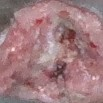
\includegraphics[width=.3\linewidth]{./Graphics/expdfu.jpg}
	\end{subfigure}
	\begin{subfigure}
		\centering
		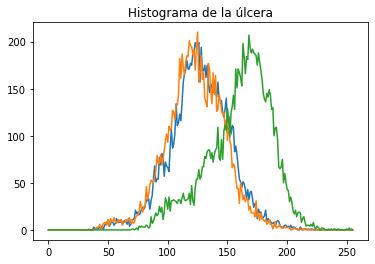
\includegraphics[width=.5\linewidth]{./Graphics/histDFU.png}
	\end{subfigure}
	\begin{subfigure}
		\centering
		
\includegraphics[width=.3\linewidth]{./Graphics/floor.jpg}
	\end{subfigure}
	\begin{subfigure}
		\centering
		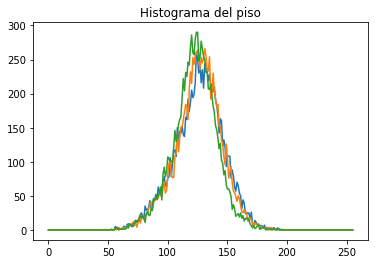
\includegraphics[width=.5\linewidth]{./Graphics/histFloor.png}
	\end{subfigure}
	\caption{Zonas confusas: (arriba) la úlcera y su histograma, (abajo) piso y su histograma}
	\label{fig:confussion}
\end{figure}

Otra de las regiones de confusión para el algoritmo es el pañuelo verde que se coloca en las consultas para realizar las curas y tomar las muestras (Figura \ref{fig:tissueMask} (izquierda)). Al ocasionar problemas el pañuelo, se decidió eliminarlo de las imágenes utilizando segmentación de umbral en los colores del pañuelo. 

\begin{figure}
	\centering
	\begin{subfigure}
		\centering
		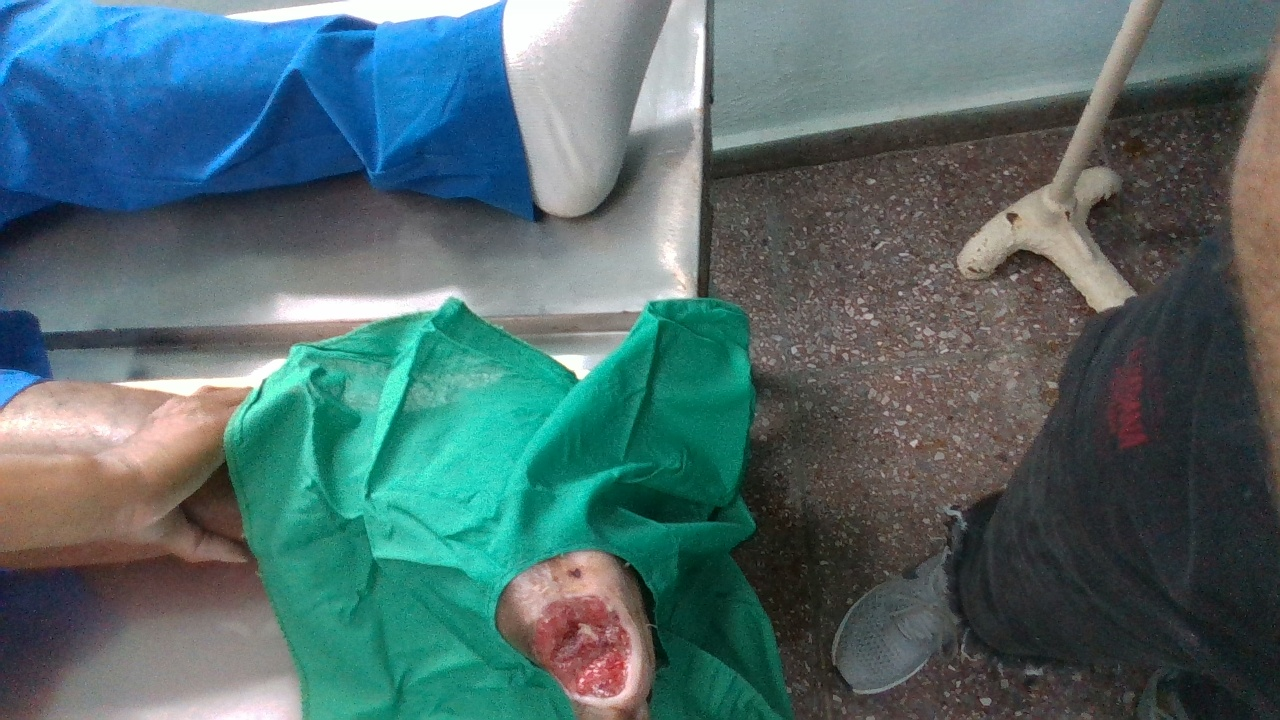
\includegraphics[width=.4\linewidth]{./Graphics/tissue.jpg}
	\end{subfigure}
	\begin{subfigure}
		\centering
		
\includegraphics[width=.4\linewidth]{./Graphics/tissueMask.jpg}
	\end{subfigure}
	\caption{Imagen donde se observa el pañuelo verde (Izquierda) y la máscara de segmentación (Derecha)}
	\label{fig:tissueMask}
\end{figure}

Para evitar estos problemas se decidió utilizar un enfoque asistido de segmentación en el cual el especialista define la región de interés para el algoritmo, o sea, recorta la imagen de forma que solo quede la úlcera en su centro. Además, se utiliza la mejora de contraste, el filtro de \textit{sharpening} para acentuar los bordes de las imágenes y la eliminación del pañuelo. Se obtienen las métricas que se muestran en la tabla siguiente.

\begin{table}[ht]
	\centering
	\begin{tabular}{lll}
		\hhline{===}
		& INACV\\
		\hhline{===}
		Jaccard medio & 84.55 \% \\ \hline
		F1-Score medio & 88.29 \% \\ \hline
		Precisión media& 88.04 \% \\
		\hline
		Recobrado medio & 91.54 \\
		\hline
	\end{tabular}
	\caption{Métricas de evaluación de la segmentación en el conjunto de datos obtenidos en el INACV}
	\label{tab:metricSegm}
\end{table}

Como alternativa al enfoque asistido de segmentación se experimentó la alternativa propuesta en~\cite{filko2018wound}. Este método propone construir subimágenes de tamaño 16 $\times$ 16 de cada \textit{frame} y entrenar el algoritmo kNN con la distancia de Bhattacharyya y $k = 7$ para predecir la localización de la úlcera. Pero debido a los problemas referidos a las zonas de confusión no dió resultados admisibles. Otro de los enfoques con los que se experimentó es utilizar las imágenes de profundidad para eliminar el ruido en las imágenes RGB. Este enfoque se probó pero no arrojó de igual manera resultados concluyentes. Por estas razones se decidió por la alternativa asistida y el algoritmo de seguimiento de objetos en secuencias de vídeo.

\subsection{Optimización del uso de la memoria RAM}

Todo el proceso de experimentación de la segmentación se desarrolló en \textit{Google Colab} haciendo uso de las Unidades Gráficas de Procesamiento (GPU). Al ejecutar la implementación utilizando los ordenadores disponibles, se enfrentó un problema de sobrecarga de la memoria RAM de los dispositivos, 8 y 16 gigabytes respectivamente.

La implementación que ocasionaba la sobrecarga almacenaba en memoria las 10 redes neuronales con los pesos correspondientes a la segmentación. Esto traía consigo que el programa en los dispositivos que se tienen a disposición se cerrara debido al llenado de la RAM. Se cambió dicha implementación a cambio de sacrificar la velocidad de cómputo.

El cambio que se introdujo es la carga de las redes neuronales y sus pesos, uno a la vez en demanda, o sea, cuando se necesita la red $i$-ésima para realizar la predicción se carga a la memoria. De esta forma, se reduce el consumo de la RAM garantizando que exista solo una red en un momento dado y es la que se va a utilizar.

\section{Resultados y detalles de la implementación de la reconstrucción 3D}\label{sec:resRec3d}

Para realizar la reconstrucción, el algoritmo propuesto utiliza hiperparámetros que influyen al momento de generar la malla. Para cada paso de la reconstrucción se analizaron los valores con los que se optimizaba el proceso en cuanto a calidad de la malla y tiempo de ejecución.

\subsection{Creación de fragmentos}

En el primer paso de la reconstrucción se crean los fragmentos, para esto es necesario indicar cada cuantos \textit{frames} se va a generar un fragmento, por lo que se introduce el parámetro \verb|n_frames_per_fragment|. Las muestras tomadas en el INACV varían entre 40 y 80 \textit{frames}. Se observa además, que el procedimiento obtiene mejores resultados con 3-4 fragmentos, de aquí que se estime la creación de un fragmento cada 20 $frames$.

Se introduce también el parámetro \verb|max_depth|, los valores de profundidad mayores que \verb|max_depth| serán truncados a cero. Teniendo en cuenta que las muestras se obtienen a una distancia de $20\text{cm}$ a $30\text{cm}$, se puede estimar este valor como $85\text{cm}$.

La odometría RGBD calcula el movimiento de la cámara entre dos imágenes RGBD consecutivas, en \textit{Open3D} se encuentran disponibles dos métodos:~\cite{steinbrucker2011real} y~\cite{park2017colored}, siendo este último el que mejores resultados obtiene en la mayoría de los conjuntos de datos. En el dominio de la imagen de profundidad, si dos píxeles alineados tienen una diferencia de profundidad menor que un valor especificado, se considera una correspondencia. Un valor más grande induce una búsqueda más agresiva, pero es propenso a resultados inestables. De aquí se deduce otro parámetro útil \verb|max_depth_diff|, con un valor de $3\text{mm}$.

Para finalmente generar el volúmen TSDF del fragmento, se necesita precisión, por lo que se precisan \textit{voxels} de 1mm aproximadamente, para esto se define el tamaño del TSDF cúbico a 0.5m, con lo que se obtiene $\frac{0.5\text{mm}}{512}$ aproximadamente 1mm.

\subsection{Registro y refinamiento de fragmentos}

Para preprocesar los fragmentos como nubes de puntos se reduce la muestra a un nuevo tamaño de voxel, se llama a este parámetro como \verb|voxel_size|. Aquí nuevamente se busca precisión, por lo que se intenta no reducir la muestra y asignar el valor real de 1mm, y este será el valor usado para todos los procesos posteriores.

En \textit{Open3D} se tienen dos procedimientos disponibles para el registro ICP: \textit{punto a punto}~\cite{besl1992method}  y \textit{punto a plano}~\cite{chen1992object}, en~\cite{rusinkiewicz2001efficient} se muestra que el algoritmo \textit{punto a plano} para ICP converge con mayor rapidez que \textit{punto a punto}. Recientemente, en~\cite{park2017colored} se introduce una variante para ICP, que usa tanto las características geométricas como el color para el registro, la información de color cierra la alineación a lo largo del plano tangente. Por lo tanto, este algoritmo es más preciso y más robusto que los algoritmos de registro de nubes de puntos anteriores, mientras que la velocidad de ejecución es comparable a la del registro ICP. Luego el parámetro \verb|icp_method| apuntará al último algoritmo descrito.

Tanto el registro ICP como la variante vista anteriormente se conocen como métodos de registro local porque se basan en una alineación aproximada como inicialización. Existe otra clase de métodos de registro, conocida como registro global. Esta familia de algoritmos no requiere una alineación para la inicialización. Por lo general, producen resultados de alineación menos estrictos y se utilizan como inicialización de los métodos locales. La elección de este método se debate entre RANSAC y Registro Global Rapido (FGR) introducido en~\cite{zhou2016fast}. La solución de registro global basada en RANSAC puede llevar mucho tiempo debido a las innumerables propuestas y evaluaciones de modelos. En~\cite{zhou2016fast} se introdujo un enfoque más rápido que optimiza rápidamente los pesos de proceso de línea de pocas correspondencias. Como no hay una propuesta de modelo ni una evaluación para cada iteración, el enfoque propuesto en~\cite{zhou2016fast} puede ahorrar mucho tiempo computacional. Con la configuración apropiada, la exactitud de FGR es incluso comparable a ICP, se pueden observar mas resultados en~\cite{zhou2016fast}.

\section{Resultados de los experimentos relativos a la medición de las UPD}

En la etapa de medición de las úlceras de pie diabético era necesario evaluar la precisión de las mediciones a través de los modelos tridimensionales obtenidos con las cámaras de profundidad y el proceso de reconstrucción. 

\subsection{Generación de tapas para las UPD}

La generación de las tapas de las úlceras de pie diabético constituyen un paso importante en el algoritmo para la estimación del volumen de la misma. La implementación del algoritmo de generación consiste en la detección de los puntos del borde de la malla poligonal de la úlcera que se asume coinciden con los bordes de la úlcera. Estos puntos se detectan anulando la componente $z$ de los puntos de la malla, luego se calcula la envoltura convexa de la imagen plana y los bordes son aquellos puntos que se localicen sobre la envoltura convexa. Posteriormente, se aplica un \textit{spline} cúbico para interpolar la superficie de la tapa.

Se definen dos tipos de úlceras teniendo en cuenta la forma de la cavidad, con el fin de explicar los resultados de la generación de las tapas, para ello se toma como referencia un plano imaginario ($T_P$) que se traza interpolando los puntos del borde de la UPD:

\begin{itemize}
	\item \textit{Cóncavas:} aquellas úlceras en las cuales la superficie de su tapa se puede aproximar por un plano, debido a que la mayor parte de la úlcera está por debajo de $T_P$.(Figura \ref{fig:planar} (izquierda)).
	\item \textit{Convexas:} aquellas úlceras en las cuales la superficie de su tapa no se puede aproximar por un plano, debido a que la mayor parte de la UPD está por encima de $T_P$. (Figura \ref{fig:planar} (derecha)).
\end{itemize}

\begin{figure}[ht]
	\centering
	\begin{subfigure}
		\centering
		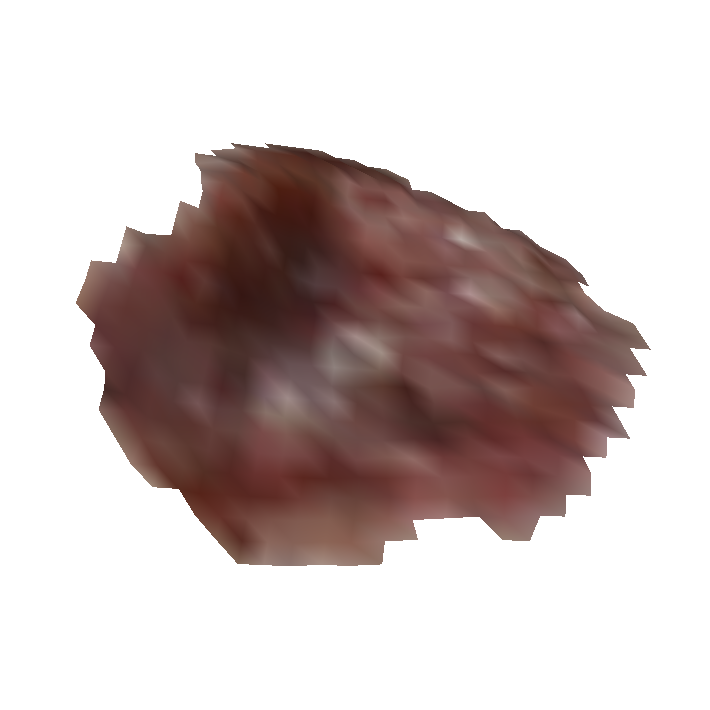
\includegraphics[width=.25\linewidth]{./Graphics/planar.png}
	\end{subfigure}
	\begin{subfigure}
		\centering
		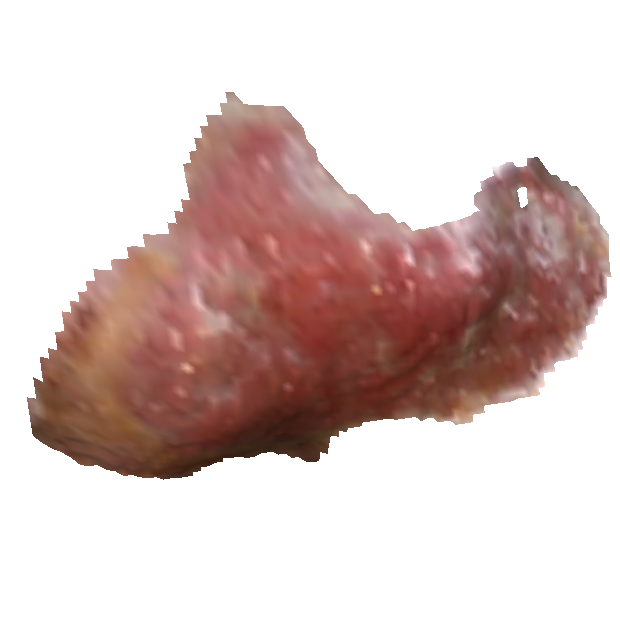
\includegraphics[width=.25\linewidth]{./Graphics/noPlanar.png}
	\end{subfigure}
	\caption{Tipos de UPD según la forma de su cavidad: (izquierda) UPD cóncava, (derecha) UPD convexa.}
	\label{fig:planar}
\end{figure}

Se tomaron 10 úlceras del conjunto de datos, de pacientes distintos para realizar experimentos sobre la generación de la tapa. Este experimento se evalúa con información brindada por los especialistas sobre la superficie de cicatrización y granulación de las UPD, debido a que no se cuenta con las superficies verdaderas de las tapas.

Las tapas obtenidas para úlceras cóncavas estiman bastante bien la superificie (Figura \ref{fig:planartops}), pues cubren toda la úlcera y se trazan cercanas al nivel que alcanzaría la cicatrización y granulación de la lesión. Sin embargo, con las úlceras convexas no se obtienen resultados satisfactorios (Figura \ref{fig:noplanartops}). 

\begin{figure}[ht]
	\centering
	\begin{subfigure}
		\centering
		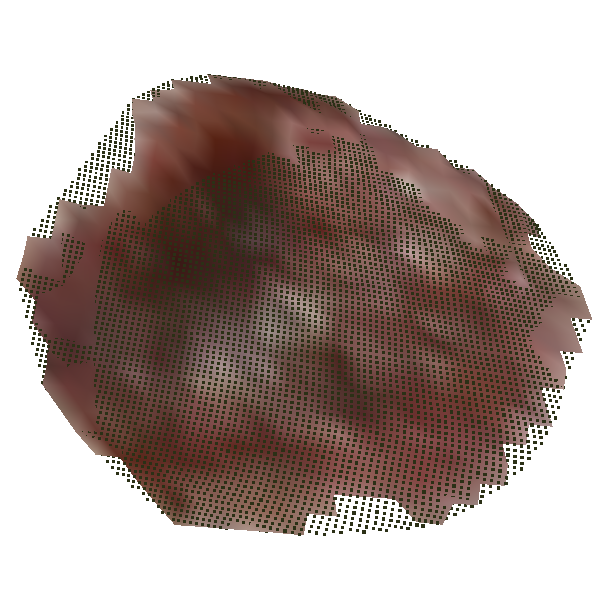
\includegraphics[width=.2\linewidth]{./Graphics/planar01.png}
	\end{subfigure}
	\begin{subfigure}
		\centering
		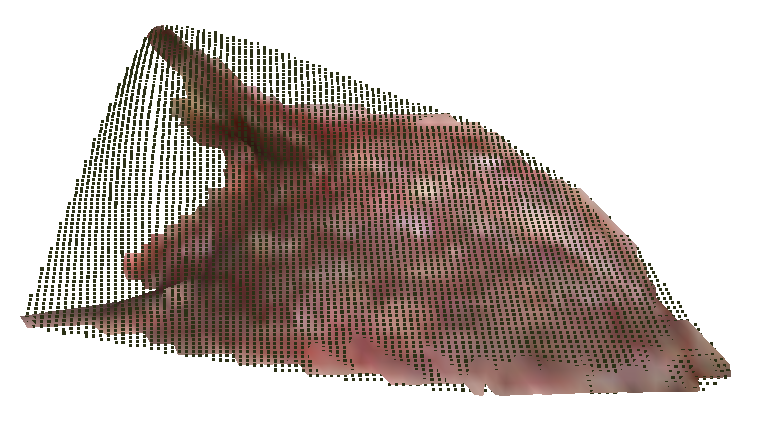
\includegraphics[width=.2\linewidth]{./Graphics/planar03.png}
	\end{subfigure}
	\begin{subfigure}
		\centering
		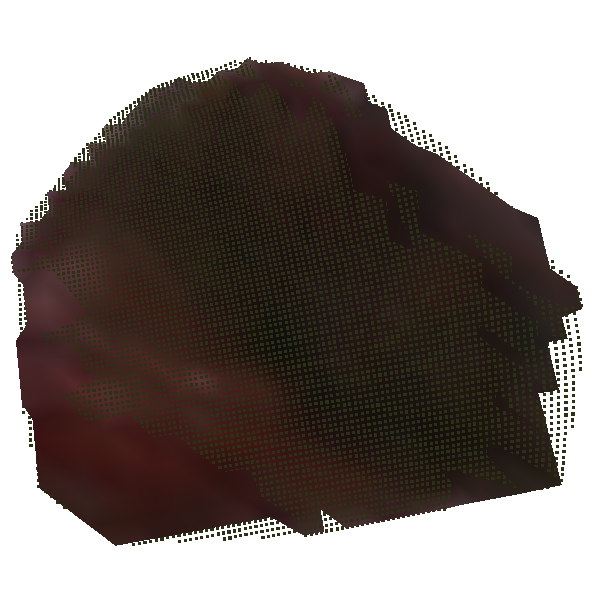
\includegraphics[width=.2\linewidth]{./Graphics/planar02.png}
	\end{subfigure}
	\begin{subfigure}
		\centering
		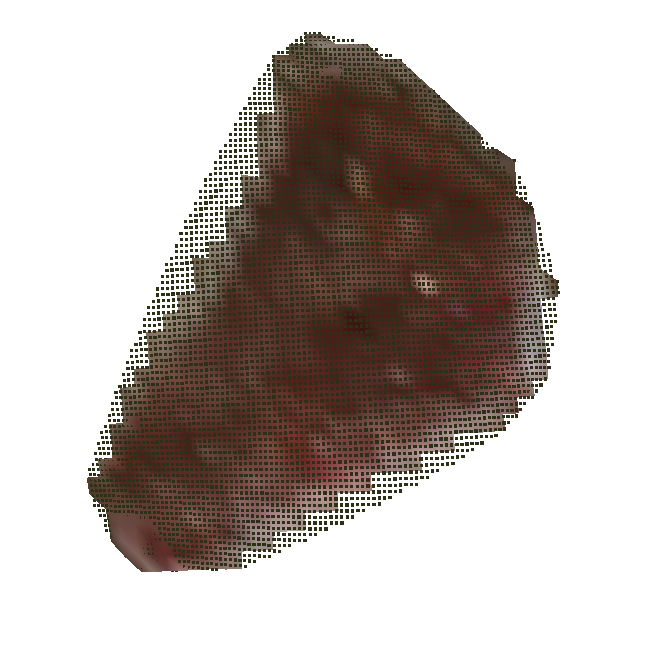
\includegraphics[width=.2\linewidth]{./Graphics/planar04.png}
	\end{subfigure}
	\caption{Estimación de la tapa de úlceras cóncavas.}
	\label{fig:planartops}
\end{figure} 

\begin{figure}[ht]
	\centering
	\begin{subfigure}
		\centering
		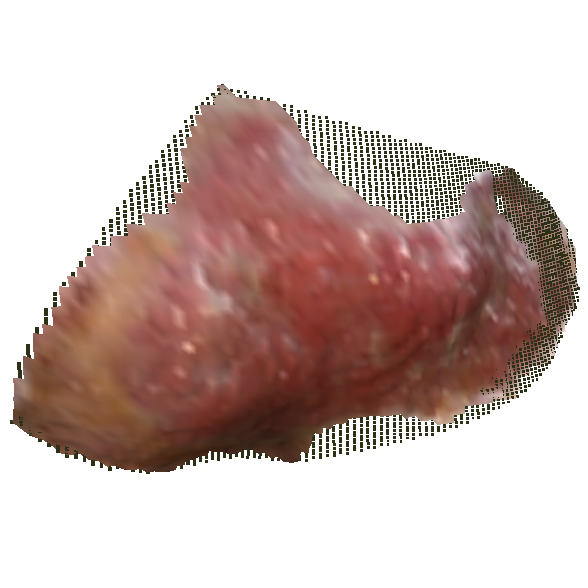
\includegraphics[width=.2\linewidth]{./Graphics/noplanar02.png}
	\end{subfigure}
	\begin{subfigure}
		\centering
		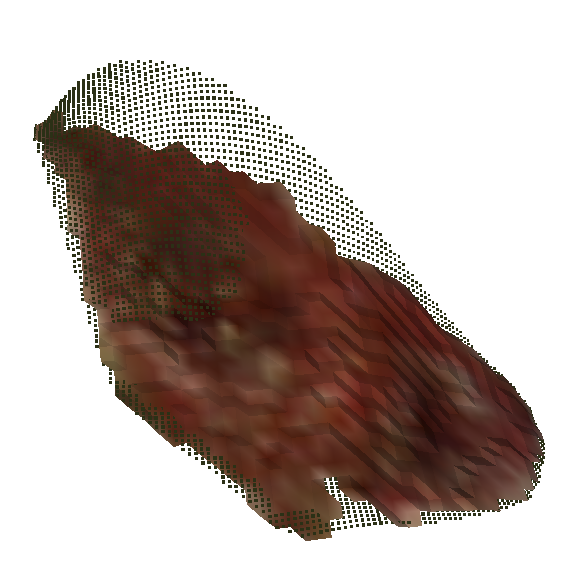
\includegraphics[width=.18\linewidth]{./Graphics/noplanar01.png}
	\end{subfigure}
	\begin{subfigure}
		\centering
		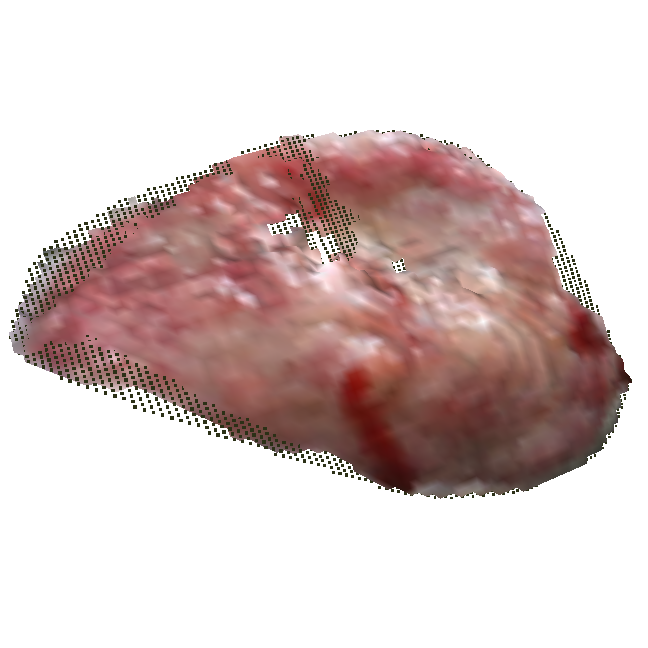
\includegraphics[width=.2\linewidth]{./Graphics/noplanar03.png}
	\end{subfigure}
	\begin{subfigure}
		\centering
		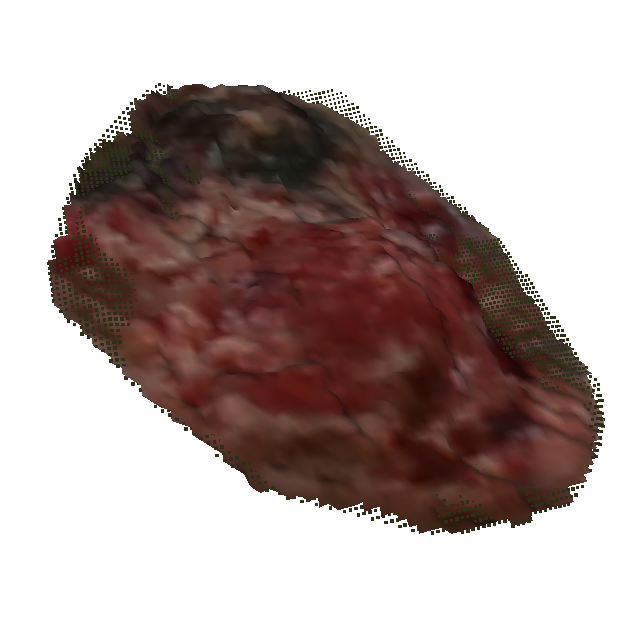
\includegraphics[width=.18\linewidth]{./Graphics/noplanar05.png}
	\end{subfigure}
	\caption{Estimación de la tapa de úlceras convexas. }
	\label{fig:noplanartops}
\end{figure} 

Esto ocurre debido a que la interpolación se ejecuta solo con los datos del borde de la úlcera lo que no aporta información de relativa a la ubicación de la cavidad de la lesión. Por esto se exploró otra alternativa, calcular la envoltura convexa de la malla de la úlcera e interpolar sobre los puntos que se encuentran sobre la envoltura convexa. Este enfoque aporta mejores resultados en la generación de tapas, en particular en las lesiones convexas, pero aumenta el error en la medición de úlcera cóncavas y en el experimento de precisión que se describe en la Sección \ref{sec:expPrec}. Por esta razón, se decidió adoptar con el enfoque anterior priorizando las úlceras cóncavas.

\subsection{Evaluación de la precisión de las mediciones}\label{sec:expPrec}

La medición de las úlceras de pie diabético a través de la reconstrucción 3D necesita ser precisa, con el fin de validar el sistema y aportar información de valor a los especialistas que les ayude a realizar un seguimiento de la evolución del paciente. Por tanto, se realizó un experimento para evaluar la precisión del sistema en medir perímetro, área y volumen. 

Para la experimentación es necesario poseer datos acerca del valor numérico real de los estimadores geométricos de una o varias úlceras. Debido a la inexistencia de los datos o un método para la medición, se utilizó como objeto una pieza de poliespuma con una cavidad con forma de cilindro circular recto de diámetro de $d = 4$cm y altura $h = 1.1$cm (Figura \ref{fig:recObj}). Los valores numéricos de las mediciones reales del objeto son:

\begin{itemize}
	\item Perímetro ($P$): la cavidad tiene forma de circunferencia, por tanto, se calcula $P = P_{circ} = 2\pi r$ donde $r$ es el radio de la circunferencia. Por tal razón, el perímetro es $$P = 2\pi * 20\text{mm} = 40\pi\text{mm}$$
	\item Área ($A$): la cavidad tiene forma de cilindro circular recto, por tanto, su área se calcula como el área total de la superficie menos el área de la base del cilindro. La ecuación quedaría:
	$$A = A_{cil_{L}} + A_{cil_{B}} =  2\pi rh + \pi r^2 = 440 \pi \text{mm}^2 + 400\pi \text{mm}^2 = 840 \pi\text{mm}^2$$ 
	\item Volumen ($V$): la cavidad es un cilindro circular recto, por tanto, se calcula $$V = V_{cil} = \pi r^2 h = 400\pi 
	* 11 \text{mm}^3 = 4400\pi \text{mm}^3$$
\end{itemize}

Estos valores se obtuvieron midiendo de forma directa el diámetro y la altura del objeto, luego, aplicando las fórmulas geométricas correspondientes. 

\begin{figure}[ht]
	\centering
	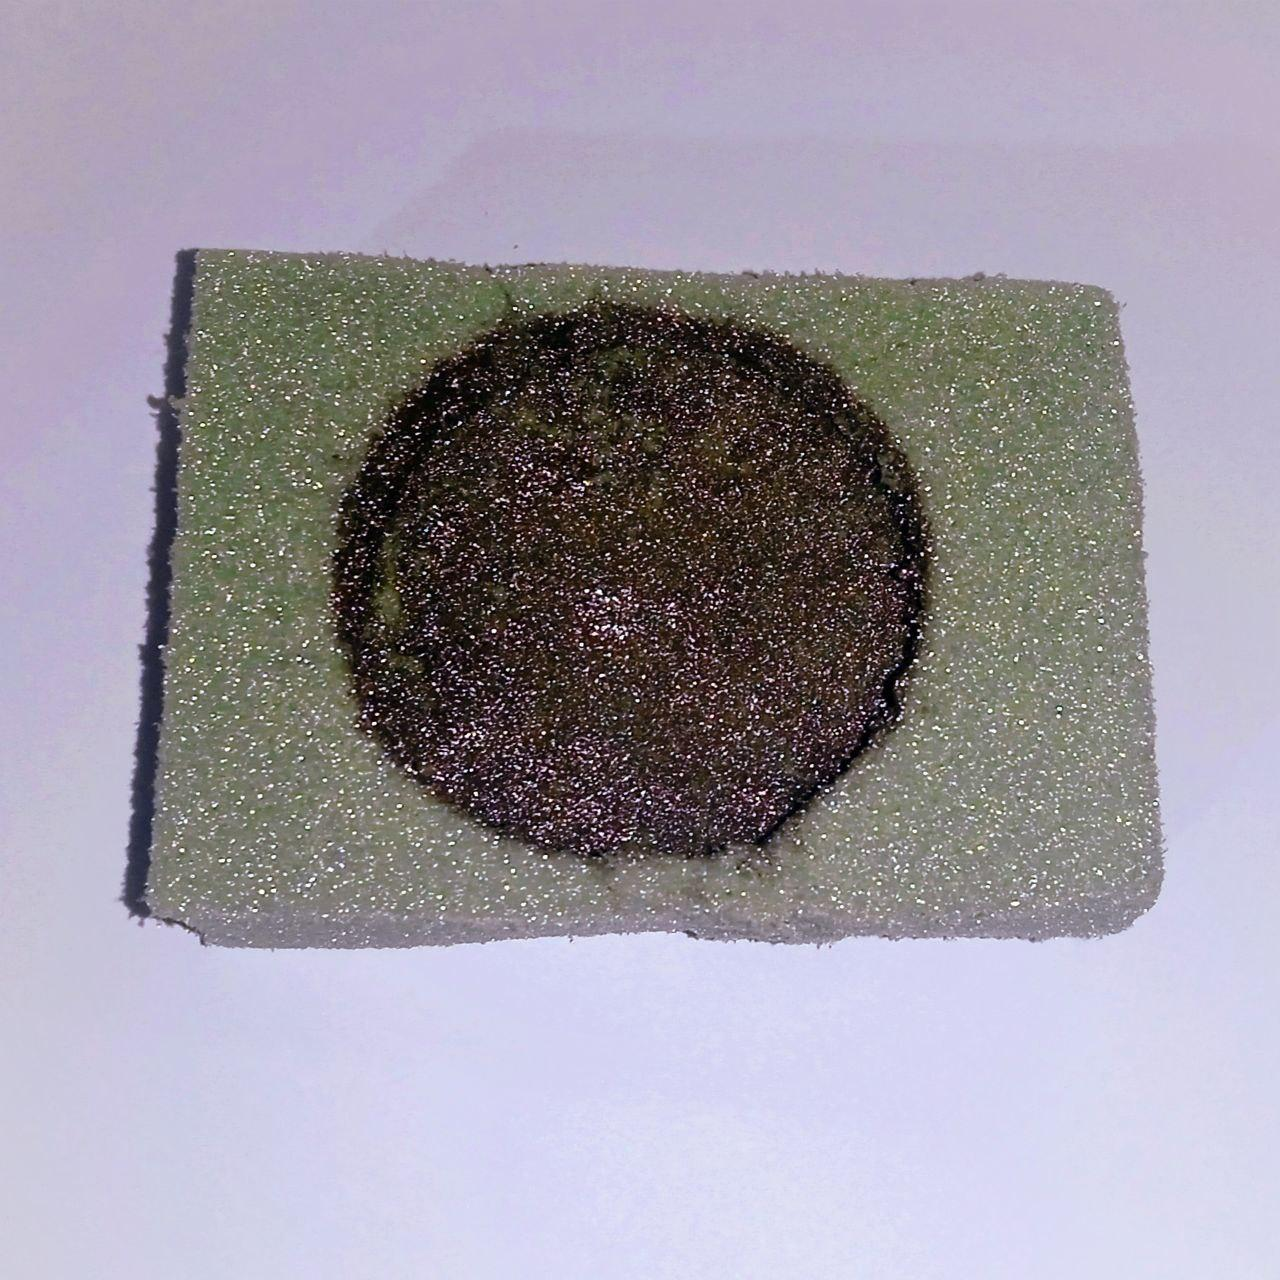
\includegraphics[width=4cm]{./Graphics/reconstruction-object.jpg}
	\caption{Objeto de prueba del experimento}
	\label{fig:recObj}
\end{figure}

El experimento consiste en realizar la reconstrucción 3D del objeto para obtener su modelo, medir y luego, comparar con los valores numéricos reales para calcular el error cometido. Es necesario conocer también la estabilidad de la medición, esto es que al realizar el proceso sobre el mismo objeto siempre se cometa el mismo error de aproximación. Por tal razón, se añade al experimento una etapa en la que se repite el proceso descrito anteriormente una cantidad $n$ de veces y luego se halla la media y desviación estándar del error cometido en cada instancia del experimento.

Se tomaron $n = 20$ secuencias de vídeo RGB-D haciendo distintos recorridos, comenzando la secuencia en diferentes puntos de vista y a diferentes distancias del objetivo siempre manteniendo el rango recomendado. Se realizaron las reconstrucciones correspondientes de la escena, obteniéndose los modelos 3D. De forma manual, se eliminaron de los modelos aquellos vértices que no corresponden a la zona de la cavidad. Posteriormente, se procedió a medir perímetro, área y volumen. 

Los resultados del experimento se describen a continuación. Se tomó como valor de la constante matemática $\pi$ la aproximación que brinda la implementación de \textit{Numpy} en la versión 1.23.3. Se analizan los resultados en cada uno de los estimadores.

\subsubsection{Perímetro}

En la aproximación del perímetro se esperaba un resultado de $40\pi\text{mm}$ que es $125.66370614359172\text{mm}$. Se obtuvo un error absoluto ($\epsilon_A$) máximo de $16.3324\text{mm}$ aproximadamente, que representa un error relativo ($\epsilon_R$) de $12.9969\%$ aproximadamente; por otro lado, el error absoluto mínimo que se consiguió es de aproximadamente $1.5876\text{mm}$ lo que representa un error relativo de $1.2634\%$. El error absoluto medio es aproximadamente de $10.5401\text{mm}$ lo que representa un error relativo de $8.3876\%$, la mediana del error absoluto es aproximadamente de $11.0085\text{mm}$ que representa un error relativo de un $8.7603\%$. La Figura \ref{fig:histP} muestra el histograma de frecuencias de las mediciones del perímetro y el error absoluto.

\begin{figure}[ht]
	\centering
	\begin{subfigure}
		\centering
		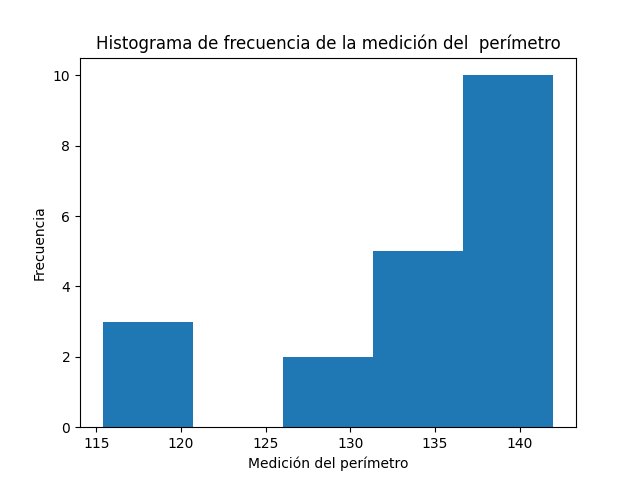
\includegraphics[width=.49\linewidth]{./Graphics/histP.png}
	\end{subfigure}
	\begin{subfigure}
		\centering
		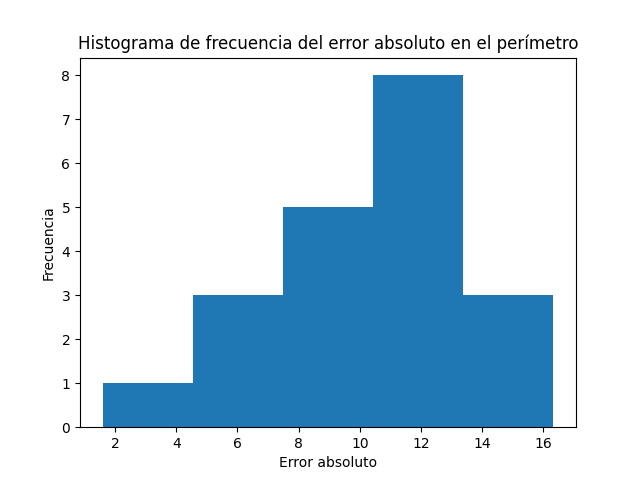
\includegraphics[width=.49\linewidth]{./Graphics/histPEA.png}
	\end{subfigure}
	\caption{Histogramas de frecuencia correspondientes al análisis de la medición del perímetro. (Izquierda) histograma de la medición y (Derecha) histograma del error absoluto.}
	\label{fig:histP}
\end{figure}

Como se observa en la Figura \ref{fig:histP} (Izquierda) la tendencia en la muestra es estimar el perímetro por encima del valor real. El intervalo de confianza de la media del error relativo es $[7.0835\%, 9.6916\%]$ con $\alpha =0.95$. Por esta razón se concluye que el error relativo que se comete al aproximar el perímetro es de $8.3876\% \pm 1.3040\%$. 

Luego, al analizar la dispersión de las mediciones se encuentra que la media de las aproximaciones es $133.5361\text{mm}$ que contiene $\epsilon_R=6.2646\%$ y la desviación típica con respecto a esta media es $7.7953\text{mm}$. Por tal razón, en un conjunto de mediciones de una misma úlcera se puede concluir que se van a obtener valores con desviación estándar $7.7953\text{mm}$ de la media que ya tiene un error de aproximación descrito anteriormente.

\subsubsection{Área}


En la aproximación del área del objeto se esperaba un resultado de $840\pi\text{mm}^2$ que es $2638.9378290154264\text{mm}^2$. Se obtuvo un error absoluto ($\epsilon_A$) máximo de aproximadamente $1300.6449\text{mm}^2$, que representa un error relativo ($\epsilon_R$) de $49.2866\%$ aproximadamente; por otro lado, el error absoluto mínimo que se consiguió es de aproximadamente $8.0087\text{mm}^2$ lo que representa un error relativo de $0.3034\%$. El error absoluto medio es aproximadamente de $470.9007\text{mm}^2$ lo que representa un error relativo de $17.8443\%$, la mediana del error absoluto es aproximadamente de $428.6708\text{mm}^2$ que representa un error relativo de un $16.2440\%$. La Figura \ref{fig:histA} muestra el histograma de frecuencias de las mediciones del área y el error absoluto.

\begin{figure}[ht]
	\centering
	\begin{subfigure}
		\centering
		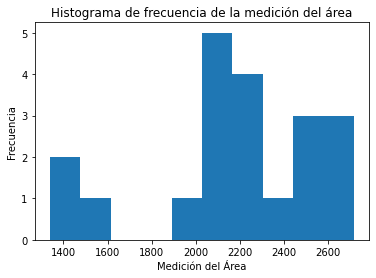
\includegraphics[width=.49\linewidth]{./Graphics/histA.png}
	\end{subfigure}
	\begin{subfigure}
		\centering
		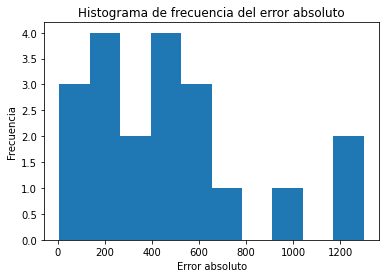
\includegraphics[width=.49\linewidth]{./Graphics/histAEA.png}
	\end{subfigure}
	\caption{Histogramas de frecuencia correspondientes al análisis de la medición del área. (Izquierda) histograma de la medición y (Derecha) histograma del error absoluto.}
	\label{fig:histA}
\end{figure}

Como se observa en la Figura \ref{fig:histA} (Izquierda) la tendencia en la muestra es estimar el área por debajo del valor real. El intervalo de confianza de la media del error relativo es $[11.3237\%, 24.3648\%]$ con $\alpha =0.95$. Por esta razón se concluye que el error relativo que se comete al aproximar el área es de $17.8443\% \pm 6.5205\%$. 

Luego, al analizar la dispersión de las mediciones se encuentra que la media de las aproximaciones es $2181.3191\text{mm}^2$ que contiene $\epsilon_R=17.3410\%$ y la desviación típica con respecto a esta media es $375.1690\text{mm}^2$. Por tal razón, en un conjunto de mediciones de una misma úlcera se puede concluir que se van a obtener valores con desviación estándar $375.1690\text{mm}^2$ de la media que ya tiene un error de aproximación descrito anteriormente.

\subsubsection{Volumen}

En la aproximación del volumen se esperaba un resultado de $4400\pi\text{mm}^3$ que es $13823.00767579509\text{mm}^3$. Se obtuvo un error absoluto ($\epsilon_A$) máximo de aproximadamente $7421.2339\text{mm}^3$, que representa un error relativo ($\epsilon_R$) de $53.6875\%$ aproximadamente; por otro lado, el error absoluto mínimo que se consiguió es de aproximadamente $314.7221\text{mm}^3$ lo que representa un error relativo de $2.2767\%$. El error absoluto medio es aproximadamente de $3289.5647\text{mm}^3$ lo que representa un error relativo de $23.7977\%$, la mediana del error absoluto es aproximadamente de $2672.1483\text{mm}^3$ que representa un error relativo de un $19.3311\%$. La Figura \ref{fig:histV} muestra el histograma de frecuencias de las mediciones del volumen y el error absoluto.

\begin{figure}[ht]
	\centering
	\begin{subfigure}
		\centering
		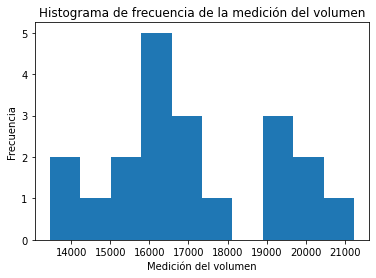
\includegraphics[width=.49\linewidth]{./Graphics/histV.png}
	\end{subfigure}
	\begin{subfigure}
		\centering
		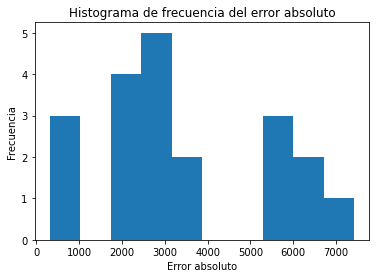
\includegraphics[width=.49\linewidth]{./Graphics/histVEA.png}
	\end{subfigure}
	\caption{Histogramas de frecuencia correspondientes al análisis de la medición del volumen. (Izquierda) histograma de la medición y (Derecha) histograma del error absoluto.}
	\label{fig:histV}
\end{figure}

Como se observa en la Figura \ref{fig:histA} (Izquierda) la tendencia en la muestra es estimar el volumen por encima del valor real. El intervalo de confianza de la media del error relativo es $[16.7570\%, 30.8384\%]$ con $\alpha =0.95$. Por esta razón se concluye que el error relativo que se comete al aproximar el área es de $23.7977\% \pm 7.0407\%$. 

Luego, al analizar la dispersión de las mediciones se encuentra que la media de las aproximaciones es $17043.4887\text{mm}^3$ que contiene $\epsilon_R=23.2979\%$ y la desviación típica con respecto a esta media es $2134.9136\text{mm}^3$. Por tal razón, en un conjunto de mediciones de una misma úlcera se puede concluir que se van a obtener valores con desviación estándar $2134.9136\text{mm}^3$ de la media que ya tiene un error de aproximación descrito anteriormente.


\begin{table}[ht]
	\centering
	\begin{tabular}{lll}
		\hhline{===}
		& Error absoluto medio & Error relativo medio\\
		\hhline{===}
		Perímetro & $10.5401\text{mm} \pm 1.4250\text{mm}$ & $8.3876\% \pm 1.3040\%$ \\ \hline
		Área & $470.9007\text{mm}^2 \pm 172.0728\text{mm}^2$ & $17.8443\% \pm 6.5205\%$\\ \hline
		Volumen & $3289.5647\text{mm}^3 \pm 973.2375\text{mm}^3$ & $23.7977\% \pm 7.0407\%$\\
		\hline
	\end{tabular}
	\caption{Resumen del error cometido en las mediciones}
	\label{tab:err}
\end{table}


\backmatter

\begin{conclusions}

La creación de un sistema de bajo costo y no intrusivo para llevar a cabo mediciones en las UPDs es de vital importancia, pues permite brindar a los centros médicos una herramienta para el seguimiento de la evolución de los tratamientos aplicados a dicha enfermedad. En particular, esta investigación propone un sistema de reconstrucción, segmentación 3D y mediciones de perímetro, superficie y volúmen de UPDs a partir de la captura de una secuencia de imágenes RGB-D. Esto conforma el paso base para la realización de un software intuitivo que pueda ser manejado directamente por los especialistas de centros médicos cubanos.

La implementación consiste en varias etapas. Primeramente el usuario selecciona una región de interés con forma rectangular para luego comenzar con la captura de la secuencia, aplicando filtros de pre/post-procesamiento a los mapas de color y profundidad respectivamente. A continuación se procede a segmentar el conjunto de imágenes de color, usando un ensemble entre las redes neuronales LinkNet y UNet, obteniendo las máscaras binarias. Se utiliza la secuencia de la captura para la creación de fragmentos y su registro global, para luego integrar la escena usando las imágenes segmentadas. Como resultado, se obtiene una malla de la cual solo tomamos la región con color. Por último se procede a tomar mediciones a la malla resultante.

Como resultado final, se alcanzó un error absoluto de aproximadamente 10mm para el cálculo de perímetro, mientras que para el área y volumen se alcanzaron valores de $470mm^2$ y $3289mm^3$. Se observa como en medidas de mayor dimensión tienden a aumentar los errores, sin embargo, los resultados obtenidos lucen prometedores ante trabajos futuros. A continuación, se proponen un conjunto de recomendaciones y mejoras para posteriores investigaciones, esperando la satisfactoria continuidad de este proyecto.
\end{conclusions}

\begin{recomendations}
	
Uno de los principales problemas enfrentados durante esta investigación fue la segmentación de la región ulcerosa con un método automático, rápido  y que consuma bajos recursos de procesamiento, se desarrollaron varios enfoques que funcionaron pero a cambio de la velocidad de cómputo y la asistencia de los especialistas para reducir el ruido del ambiente. Por esto una de las recomendaciones para futuros trabajos es la investigación de métodos investigativos que cumplan las tres característica. El algoritmo ideal, sería aquel que permita segmentar en tiempo real la zona de la úlcera, para así poder utilizar algoritmos de reconstrucción en tiempo real.

Por otro lado, se utilizó un algoritmo de reconstrucción 3D a posteriori, donde se fijaban los parámetros descritos en la Sección \ref{sec:resRec3d}. Se recomienda investigar algoritmos de selección automática de parámetros para obtener mejores resultados en la reconstrucción y para agilizar el tiempo de cómputo de este proceso.

Posterior a la reconstrucción se desarrolló un proceso de medición de la región ulcerosa. En la medición del volumen se ejecuta el proceso de generación de tapas a la cavidad. Como se presentó en los resultados los enfoques adoptados no cumplen las restricciones para las úlceras convexas o no mantienen la tasa de error en un margen adecuado. Por esto se sugiere investigar otros enfoques en la generación de tapas a la cavidad, utilizando otros métodos de interpolación o técnicas de aprendizaje de máquinas o aprendizaje profundo.

La implementación de todo el software se desarrolló en Python como lenguaje de programación. Este lenguaje es el más utilizado para la construcción de prototipos como es el caso, pero no para sistemas que sean utilizados en producción y se necesite rapidez. Por esta razón se recomienda implementar el sistema en un lenguaje como C++. Además, se recomienda desarrollar una interfaz visual amigable para los especialistas en angiología, así como añadir al sistema una base de datos que les permita almacenar los datos del paciente y tener un seguimiento del porciento de granulación y cicatrización de la úlcera de forma automatizada.
\end{recomendations}

\DeclareFieldFormat{labelnumberwidth}{\mkbibbrackets{#1}}

\defbibenvironment{bibliography}
  {\list
     {\printtext[labelnumberwidth]{%
      \printfield{labelprefix}%
      \printfield{labelnumber}}}
     {\setlength{\labelwidth}{\labelnumberwidth}%
      \setlength{\leftmargin}{\labelwidth}%
      \setlength{\labelsep}{\biblabelsep}%
      \addtolength{\leftmargin}{\labelsep}%
      \setlength{\itemsep}{\bibitemsep}%
      \setlength{\parsep}{\bibparsep}}%
      \renewcommand*{\makelabel}[1]{\hss##1}}
  {\endlist}
  {\item}

\printbibliography

\end{document}